\chapter{鞍点的处理}
\label{chap:saddle-points}

一个算法运行结束，报告梯度范数只有$0.06$。这句话能说明什么？地面在这里几乎是平的，可是平的地方不止谷底，山顶和山口也是平的。下降算法走到山口附近，脚下坡度变得很小，步子随之变小，看起来像是快要到达终点，其实旁边还有一条向下的路。

非凸目标里，这种情形不是例外。第~\ref{chap:first-order-methods}章到第~\ref{chap:trust-region}章的保证，多数只说梯度趋于零。本章追问这以后的事：梯度已经很小时，怎样知道目标还能不能继续下降，怎样真正下降，最后又能声称得到了什么样的点。

全章用同一个二维目标把这些问题算到底。先把梯度为零的点分类，看清二阶信息能排除什么、还留下什么。然后讨论怎样只靠Hessian向量积找到向下弯曲的方向，并分清“找到”和“没有找到”分别能得出什么结论。

接着比较三种离开的办法：已知向下弯曲的方向时沿它走一步；只有梯度时给迭代点一点随机扰动；手里有二次模型时保留它的不定性。最后把停止条件和计算成本放在一起，说明一次运行究竟可以报告什么样的保证。

\section{驻点的类型}
\label{sec:saddle-types}

梯度为零的点有哪几类，二阶信息能把它们分开到什么程度？先用一个具体的目标看清这些点的样子，再给定义，然后专门讨论二阶信息判断不了的情形。

\paragraph{贯穿全章的例子}
我们用下面这个目标，它在$x_1$方向是一口双井，在$x_2$方向是一只碗：
\begin{equation}
 f(\bm{x})=\frac14\bigl(x_1^2-1\bigr)^2+\frac12x_2^2.
 \label{eq:saddle-example}
\end{equation}
它的梯度和Hessian可以直接写出：
\begin{equation}
 \nabla f(\bm{x})=\begin{bmatrix}x_1^3-x_1\\x_2\end{bmatrix},\qquad
 \nabla^2 f(\bm{x})=\begin{bmatrix}3x_1^2-1&0\\0&1\end{bmatrix}.
 \label{eq:saddle-example-derivatives}
\end{equation}

令梯度为零，第二个分量给出$x_2=0$，第一个分量给出$x_1(x_1^2-1)=0$。于是有三个驻点，它们的目标值和Hessian是
\[
 \begin{aligned}
 (\pm1,0):&\quad f=0,\quad \nabla^2f=\operatorname{diag}(2,1),\\
 (0,0):&\quad f=\tfrac14,\quad \nabla^2f=\operatorname{diag}(-1,1).
 \end{aligned}
\]

$f\geq0$处处成立，所以$(\pm1,0)$是全局最优解。原点沿$x_2$方向是最低点，沿$x_1$方向是最高点，这正是一个山口。图~\ref{fig:saddle-running-landscape}画出了等高线和$x_2=0$上的截面。

\begin{BookInlineFigure}
  \centering
  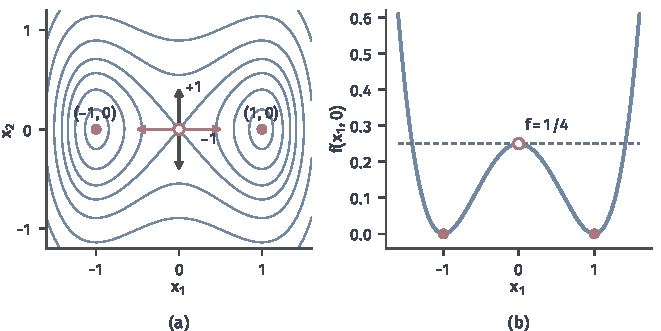
\includegraphics[width=112mm]{figures/05-optimization/02-smooth-optimization/matplotlib/saddle-running-landscape/figure.pdf}
  \caption{目标~\eqref{eq:saddle-example}。(a)蓝线是等高线，红点是两个全局最优解，空心点是原点处的鞍点，红色箭头是曲率为$-1$的方向，灰色箭头是曲率为$+1$的方向。(b)$x_2=0$上的截面，鞍点位于两口井之间的高处，函数值为$1/4$。}
  \label{fig:saddle-running-landscape}
\end{BookInlineFigure}

后面的分析要用到两个常数。Hessian~\eqref{eq:saddle-example-derivatives}的元素随$x_1$增长，全局的常数不存在，所以我们只在带形区域上讨论：
\[
 \bm{U}=\bigl\{\bm{x}\in\mathbb{R}^2:\ \lvert x_1\rvert\leq1\bigr\}.
\]

在$\bm{U}$上，$3x_1^2-1$介于$-1$与$2$之间，因此谱范数$\lVert\nabla^2f\rVert_2\leq2$，光滑常数取$L=2$。Hessian本身的变化由差值控制：
\[
 \bigl\lvert(3x_1^2-1)-(3y_1^2-1)\bigr\rvert
 =3\lvert x_1+y_1\rvert\,\lvert x_1-y_1\rvert
 \leq6\lvert x_1-y_1\rvert.
\]
所以在$\bm{U}$上，Hessian满足下面的Lipschitz条件，常数$M=6$：
\[
 \bigl\lVert\nabla^2f(\bm{x})-\nabla^2f(\bm{y})\bigr\rVert_2\leq M\lVert\bm{x}-\bm{y}\rVert_2.
\]
全章固定步长取$\alpha=1/L=1/2$。

\paragraph{三类驻点}
站在驻点上，一阶变化消失了，目标的走势由Hessian决定。由Taylor公式，对小的$\bm{h}$，
\[
 f(\bm{x}+\bm{h})-f(\bm{x})=\frac12\bm{h}^\top\nabla^2f(\bm{x})\bm{h}+o\bigl(\lVert\bm{h}\rVert_2^2\bigr).
\]
量$\bm{h}^\top\nabla^2f(\bm{x})\bm{h}$的符号回答了“沿这个方向向上弯还是向下弯”。按照能否找到向下弯的方向，驻点分成下面几类。

\begin{definition}[驻点的类型]
 \label{def:saddle-stationary}
 设$f$二阶连续可微。若点$\bm{x}$满足
 \begin{equation}
  \nabla f(\bm{x})=\bm{0},
  \label{eq:saddle-first-order}
 \end{equation}
 就称它为\term{一阶驻点}（first-order stationary point）。若还满足
 \begin{equation}
  \nabla^2f(\bm{x})\succeq\bm{0},
  \label{eq:saddle-second-order}
 \end{equation}
 就称它为\term{二阶驻点}（second-order stationary point）。若一阶驻点满足
 \begin{equation}
  \lambda_{\min}\bigl(\nabla^2f(\bm{x})\bigr)<0,
  \label{eq:saddle-strict}
 \end{equation}
 就称它为\term{严格鞍点}（strict saddle point）。
\end{definition}

一阶驻点要么是二阶驻点，要么是严格鞍点，两者互斥。名称上有一点需要留意：局部极大点也满足式~\eqref{eq:saddle-strict}，在这个约定下同样算作严格鞍点。原因是算法只关心有没有向下弯的方向，而局部极大点和山口在这一点上没有区别。

二阶条件告诉我们这些类别和局部极小点的关系。第~\ref{chap:optimization}章证明过：局部极小点必须是二阶驻点；Hessian正定的一阶驻点一定是严格局部极小点。因此严格鞍点一定不是局部极小点，而二阶驻点之中，Hessian正定的部分一定是局部极小点。

表~\ref{tab:saddle-origin-types}列出几个函数在原点的情形，它们的梯度在原点都为零。前两行是这两条结论直接判定的情形，后三行的Hessian半正定且奇异，正是二阶条件留下的缺口。

\begin{BookInlineTable}
  \centering
  \begin{tabular}{@{}lll@{}}
    \toprule
    函数 & 原点的Hessian & 原点的类型\\
    \midrule
    $x_1^2+x_2^2$ & $\operatorname{diag}(2,2)$ & 严格局部极小点\\
    $x_1^2-x_2^2$ & $\operatorname{diag}(2,-2)$ & 严格鞍点\\
    $x_1^2+x_2^4$ & $\operatorname{diag}(2,0)$ & 二阶驻点，局部极小点\\
    $x_1^2-x_2^4$ & $\operatorname{diag}(2,0)$ & 二阶驻点，不是局部极小点\\
    $x_1^4-x_2^4$ & $\bm{0}$ & 二阶驻点，不是局部极小点\\
    \bottomrule
  \end{tabular}
  \caption{原点处的几种情形。第三行与第四行的梯度和Hessian完全相同，类型却不同。}
  \label{tab:saddle-origin-types}
\end{BookInlineTable}

\paragraph{退化情形}
Hessian半正定仍不足以说明是局部极小点。比较$x_1^2+x_2^4$和$x_1^2-x_2^4$：它们在原点的函数值、梯度和Hessian完全一样，差别只在四阶项。沿$x_2$轴看，
\[
 x_1^2+x_2^4\big|_{x_1=0}=t^4,\qquad
 x_1^2-x_2^4\big|_{x_1=0}=-t^4.
\]

前者把原点托在最低处，后者从原点沿$x_2$轴一直下降。只看到二阶为止的信息，这两个函数无法分开。图~\ref{fig:saddle-stationary-zoo}用浅红色标出比原点函数值更低的区域，只要原点的任意小邻域内有浅红色，原点就不是局部极小点。

\begin{BookInlineFigure}
  \centering
  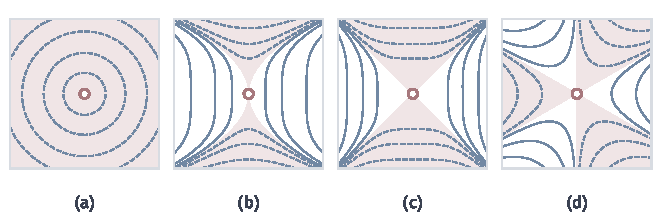
\includegraphics[width=112mm]{figures/05-optimization/02-smooth-optimization/matplotlib/saddle-stationary-zoo/figure.pdf}
  \caption{原点处四种不是局部极小点的驻点，蓝线是等高线，虚线为负值，浅红区域是函数值低于$f(\bm{0})=0$的点。(a)$-x_1^2-x_2^2$，局部极大点。(b)$x_1^2-x_2^4$，Hessian为$\operatorname{diag}(2,0)$。(c)$x_1^4-x_2^4$，Hessian为零。(d)$x_1^3-3x_1x_2^2$，Hessian为零。后三个都没有负曲率，算法靠Hessian察觉不到下降方向。}
  \label{fig:saddle-stationary-zoo}
\end{BookInlineFigure}

图中(a)的负曲率是显式的，(b)、(c)、(d)的下降则藏在更高阶的项里。(d)沿$x_1$轴的函数值是$t^3$，经过原点时由正变负，下降的一侧和上升的一侧挨在一起。

\paragraph{每条直线上都最低，仍然不是局部极小}
有人会想：既然二阶信息只看直线方向，那么补上高阶项，逐条直线检查目标是否在原点取到局部最低，总该够了吧？下面的例子说明还是不够：
\begin{equation}
 f(\bm{x})=\bigl(x_2-x_1^2\bigr)\bigl(x_2-2x_1^2\bigr).
 \label{eq:saddle-peano}
\end{equation}

展开得到$x_2^2-3x_1^2x_2+2x_1^4$，所以原点是驻点，Hessian是$\operatorname{diag}(0,2)$。先看经过原点的每条直线。沿$x_2=mx_1$，目标是
\[
 f(t,mt)=m^2t^2-3mt^3+2t^4.
\]

$m\neq0$时二次项为正，$t$足够小时函数值为正。$m=0$时是$2t^4$，沿$x_2$轴是$x_2^2$，也都大于零。所以原点在每条直线上都是严格局部最低点。

可是沿抛物线$x_2=\tfrac32x_1^2$走，两个因子一正一负：
\[
 f\bigl(t,\tfrac32t^2\bigr)=\Bigl(\tfrac12t^2\Bigr)\Bigl(-\tfrac12t^2\Bigr)=-\frac14t^4<0.
\]

原点的任意小邻域内都有比它更低的点，所以它不是局部极小点。图~\ref{fig:saddle-peano}(a)给出了几何解释：函数值为负的区域夹在两条抛物线之间，而任何一条直线在原点附近都会离开这个弯曲的窄缝。沿直线下降的想法，在这里看不到弯曲的下降路径。

\begin{BookInlineFigure}
  \centering
  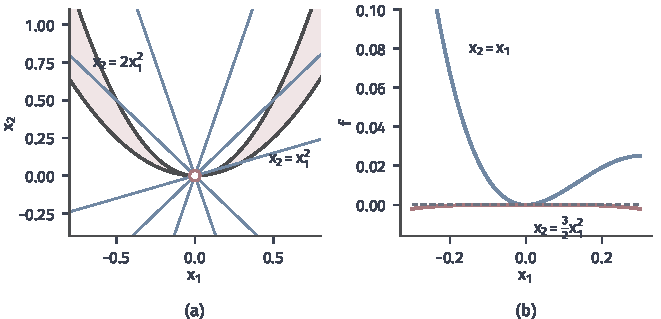
\includegraphics[width=112mm]{figures/05-optimization/02-smooth-optimization/matplotlib/saddle-peano/figure.pdf}
  \caption{目标~\eqref{eq:saddle-peano}。(a)浅红色是$f<0$的区域，夹在抛物线$x_2=x_1^2$和$x_2=2x_1^2$之间；蓝色直线在原点附近都位于这个区域之外。(b)沿直线$x_2=x_1$的函数值（蓝）在原点取最低，沿抛物线$x_2=\tfrac32x_1^2$的函数值（红）为负。}
  \label{fig:saddle-peano}
\end{BookInlineFigure}

\paragraph{二阶条件能排除什么}
把这些类别按包含关系排列，得到图~\ref{fig:saddle-class-nesting}。每往里一层，条件就强一些。

\begin{BookInlineFigure}
  \centering
  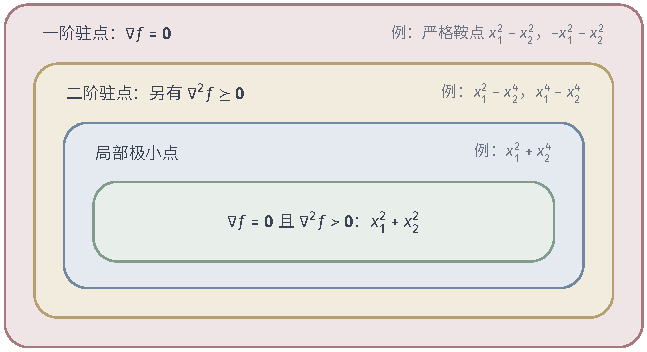
\includegraphics[width=109.6mm]{figures/05-optimization/02-smooth-optimization/tikz/saddle-class-nesting/figure.pdf}
  \caption{驻点类别的包含关系，每层右上角的函数在原点属于该层而不属于更内一层。最外层与第二层之间的差就是严格鞍点。第二层与第三层之间是退化的二阶驻点，二阶信息无法把它们和局部极小点分开。}
  \label{fig:saddle-class-nesting}
\end{BookInlineFigure}

由此可以说清楚二阶信息的能力。负特征值是确凿的证据：只要算出一个负的曲率，就能断定这里不是局部极小点。Hessian正定也是确凿的证据：这里一定是严格局部极小点。两者之间的情形，二阶信息保持沉默，并不是“大概是极小点”的意思。

所以算法的目标要说得克制。排除严格鞍点是可以做到的事，这是后面几节的内容。判定一个退化的二阶驻点是否为局部极小点，一般需要更高阶的信息，本章的方法不处理。

\paragraph{局部条件不说明全局}
上面的讨论还停留在局部。即使某点确实是局部极小点，也不说明它是全局最优解。看下面这个倾斜的双井：
\[
 \psi(x)=\frac14x^4+\frac13x^3-x^2,\qquad
 \psi'(x)=x(x-1)(x+2).
\]

三个驻点的二阶导数由$\psi''(x)=3x^2+2x-2$算出：
\[
 \psi''(0)=-2,\qquad\psi''(1)=3,\qquad\psi''(-2)=6.
\]

$x=1$是严格局部极小点，满足所有局部条件，函数值却是$-5/12$，而全局最优解$x=-2$的函数值是$-8/3$。图~\ref{fig:saddle-tilted-well}中，从$x=1$到更低的井要先翻过$x=0$处的高坡。站在黄点上，任何只依赖当地导数的判据都看不到另一口井。

\begin{BookInlineFigure}
  \centering
  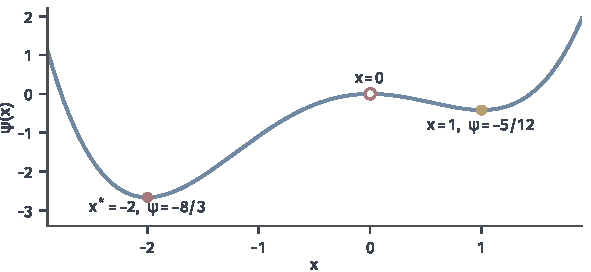
\includegraphics[width=100mm]{figures/05-optimization/02-smooth-optimization/matplotlib/saddle-tilted-well/figure.pdf}
  \caption{倾斜双井$\psi(x)=x^4/4+x^3/3-x^2$。黄点$x=1$是严格局部极小点，红点$x=-2$是全局最优解，空心点$x=0$是局部极大点。局部条件在黄点全部满足。}
  \label{fig:saddle-tilted-well}
\end{BookInlineFigure}

所以本章的“离开鞍点”只是把严格鞍点从可能的终点中排除。它既不判定退化的二阶驻点，也不保证到达全局最优解。


\section{负曲率的检测}
\label{sec:saddle-detection}

梯度已经很小时，怎样判断Hessian还有没有足够负的方向？变量很多时存不下Hessian，所以我们特别关心只用Hessian向量积能走多远，以及找到方向和没找到方向分别说明了什么。

\paragraph{要找的是什么}
对单位向量$\bm{v}$，Rayleigh商$R(\bm{v})=\bm{v}^\top\bm{H}\bm{v}$就是目标沿$\bm{v}$的曲率。谱分解$\bm{H}=\sum_i\lambda_i\bm{q}_i\bm{q}_i^\top$（特征值$\lambda_1\leq\cdots\leq\lambda_n$）给出
\begin{equation}
 \min_{\lVert\bm{v}\rVert_2=1}R(\bm{v})=\lambda_1=\lambda_{\min}(\bm{H}),
 \label{eq:saddle-rayleigh}
\end{equation}
最小值在$\bm{q}_1$处取到。

我们并不需要真的求出$\bm{q}_1$。只要有一个单位向量使$R(\bm{v})\leq-\gamma$，其中$\gamma>0$，它就是负曲率方向，后面的下降分析用到的只是这个不等式。本章的$\gamma$始终表示负曲率的大小。

在原点，$\bm{H}=\operatorname{diag}(-1,1)$，取$\bm{v}=(\cos\theta,\sin\theta)$，Rayleigh商是
\[
 R(\bm{v})=-\cos^2\theta+\sin^2\theta=-\cos2\theta.
\]
夹角在$45^\circ$以内的方向全都是负曲率方向，夹角在$30^\circ$以内的方向满足$R\leq-1/2$。图~\ref{fig:saddle-curvature-cone}显示负曲率方向占据一整个锥，这是检测能够用粗糙办法完成的原因。

\begin{BookInlineFigure}
  \centering
  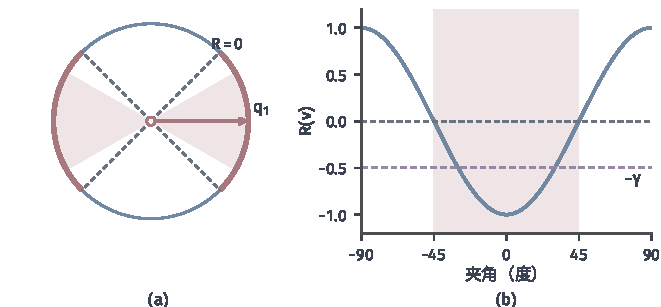
\includegraphics[width=112mm]{figures/05-optimization/02-smooth-optimization/matplotlib/saddle-curvature-cone/figure.pdf}
  \caption{$\bm{H}=\operatorname{diag}(-1,1)$的曲率随方向的变化。(a)单位圆上的红色弧是$R<0$的方向，浅红扇形是$R\leq-1/2$的方向，$\bm{q}_1$是最小特征向量。(b)$R$随方向与$\bm{q}_1$夹角的变化，浅红带是负曲率的范围，紫色虚线是阈值$-\gamma=-1/2$。}
  \label{fig:saddle-curvature-cone}
\end{BookInlineFigure}

\paragraph{矩阵存得下时}
$n$不大时，可以直接计算$\bm{H}$的特征分解，得到$\lambda_{\min}$和$\bm{q}_1$，运算量是$O(n^3)$。如果只需要回答“$\lambda_{\min}$是否大于$-\gamma$”，对$\bm{H}+\gamma\bm{I}$作Cholesky分解更省：分解成功当且仅当$\bm{H}+\gamma\bm{I}$正定，也就是$\lambda_{\min}>-\gamma$。

例中在原点取$\gamma=\tfrac12$，要分解的矩阵是
\[
 \bm{H}+\gamma\bm{I}=\operatorname{diag}\bigl(-\tfrac12,\tfrac32\bigr).
\]
第一个主元就是负的，分解失败，所以$\lambda_{\min}\leq-\tfrac12$。这种方法没有舍入以外的误差，结论是确定的，代价是要存下并分解整个矩阵。

\paragraph{矩阵存不下时}
第~\ref{chap:second-order-methods}章介绍过Hessian向量积，一次乘积的成本与一次梯度同量级。用自动微分可以精确得到它，用差分则只需要两次梯度：
\begin{equation}
 \hat{\bm{u}}=\frac{\nabla f(\bm{x}+h\bm{v})-\nabla f(\bm{x})}{h}.
 \label{eq:saddle-hvp-difference}
\end{equation}

差分带来的误差要记入账。设$\bm{v}$是单位向量，线段$[\bm{x},\bm{x}+h\bm{v}]$落在Hessian为$M$-Lipschitz的区域内。由微积分基本定理，
\[
 \nabla f(\bm{x}+h\bm{v})-\nabla f(\bm{x})-h\bm{H}\bm{v}
 =\int_0^h\bigl(\nabla^2f(\bm{x}+s\bm{v})-\nabla^2f(\bm{x})\bigr)\bm{v}\,\mathrm{d}s.
\]

被积函数的范数不超过$Ms$，积分得$Mh^2/2$。除以$h$，得到
\begin{equation}
 \lVert\hat{\bm{u}}-\bm{H}\bm{v}\rVert_2\leq\frac{Mh}{2}.
 \label{eq:saddle-hvp-error}
\end{equation}

下面用数据验证。在点$\bm{x}=\bm{0}$处取$\bm{v}=(1,1)/\sqrt2$，$h=0.1$，代入梯度~\eqref{eq:saddle-example-derivatives}，由$\nabla f(\bm{0})=\bm{0}$得到
\[
 \hat{\bm{u}}=\begin{bmatrix}h^2v_1^3-v_1\\v_2\end{bmatrix}
 \approx\begin{bmatrix}-0.7036\\0.7071\end{bmatrix},\qquad
 \bm{H}\bm{v}\approx\begin{bmatrix}-0.7071\\0.7071\end{bmatrix}.
\]
实际误差约为$0.0035$，界~\eqref{eq:saddle-hvp-error}给出$0.3$。原点左右对称，一阶误差项恰好抵消，这里的实际误差因此特别小。

图~\ref{fig:saddle-hvp-difference}换到一般的点$(0.3,0.2)$。$h$较大时误差与$h$成正比，$h$太小时舍入误差占主导，这与第~\ref{chap:second-order-methods}章的说法一致。

\begin{BookInlineFigure}
  \centering
  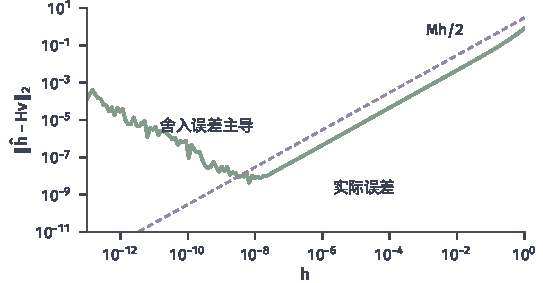
\includegraphics[width=92mm]{figures/05-optimization/02-smooth-optimization/matplotlib/saddle-hvp-difference/figure.pdf}
  \caption{目标~\eqref{eq:saddle-example}在点$(0.3,0.2)$沿$(1,1)/\sqrt2$的差分Hessian向量积误差，绿线是实际误差（双精度计算），紫色虚线是上界$Mh/2$，$M=6$。$h$小于约$10^{-8}$后舍入误差占主导。}
  \label{fig:saddle-hvp-difference}
\end{BookInlineFigure}

\paragraph{主要思想：把最小特征值变成最大特征值}
Hessian向量积最直接的用法是幂迭代：反复乘一个矩阵，向量会转向模最大的特征值所对应的方向。可是我们要的是最小特征值，而$\bm{H}$的最大模特征值可能是最大的正特征值。

解决办法是平移。设$\lVert\bm{H}\rVert_2\leq L$，令
\begin{equation}
 \bm{A}=L\bm{I}-\bm{H}.
 \label{eq:saddle-power-shift}
\end{equation}
$\bm{A}$的特征向量和$\bm{H}$相同，特征值是$a_i=L-\lambda_i\geq0$，最大的$a_1=L-\lambda_{\min}$恰好对应$\bm{H}$的最小特征值。于是对$\bm{A}$作幂迭代：
\begin{equation}
 \bm{v}^{(k+1)}=\frac{\bm{A}\bm{v}^{(k)}}{\lVert\bm{A}\bm{v}^{(k)}\rVert_2},\qquad k=0,1,\ldots
 \label{eq:saddle-power-iteration}
\end{equation}

每轮只用一次Hessian向量积。这里的上标$k$记检测内部的轮数，与外层的迭代$t$区分。把$\bm{v}^{(0)}$按特征向量展开成$\sum_ic_i\bm{q}_i$，$k$轮之后的方向正比于$\sum_ic_ia_i^k\bm{q}_i$，与$a_1$相比较小的分量按几何级数衰减。

这个迭代还有另一层含义。除以$L$之后，$\bm{A}/L=\bm{I}-\tfrac1L\bm{H}$，这正是步长$1/L$的梯度下降在二次目标上的迭代矩阵。所以幂迭代和鞍点附近的梯度下降是同一件事，第~\ref{sec:saddle-escape}节还要用到这一点。

\needspace{6\baselineskip}
\paragraph{变量}
在一个给定的点上运行检测，要维护的量是：
\begin{itemize}
 \item $\bm{v}^{(k)}\in\mathbb{R}^n$：当前的单位向量；
 \item $\bm{u}^{(k)}\in\mathbb{R}^n$：Hessian向量积$\bm{H}\bm{v}^{(k)}$；
 \item $R^{(k)}$：Rayleigh商$\langle\bm{v}^{(k)},\bm{u}^{(k)}\rangle$。
\end{itemize}

\paragraph{初始化}
选定常数$L\geq\lVert\bm{H}\rVert_2$，阈值$\gamma>0$，轮数上限$k_{\max}$，并在单位球面上均匀随机地取$\bm{v}^{(0)}$。例中在原点检测，$\bm{H}=\operatorname{diag}(-1,1)$，$L=2$，$\gamma=\tfrac12$，设随机抽到
\[
 \bm{v}^{(0)}=\frac{1}{\sqrt2}\begin{bmatrix}1\\1\end{bmatrix}.
\]

\paragraph{每轮更新}
第$k$轮依次执行以下步骤，满足结束条件时停止。

\begin{enumerate}
 \item 计算Hessian向量积$\bm{u}^{(k)}=\bm{H}\bm{v}^{(k)}$。例中第$0$轮得到
 \[
  \bm{u}^{(0)}=\frac{1}{\sqrt2}\begin{bmatrix}-1\\1\end{bmatrix}.
 \]
 \item 计算$R^{(k)}$。若$R^{(k)}\leq-\gamma$，返回$\bm{v}^{(k)}$，宣布找到了负曲率方向；若$k=k_{\max}$，宣布没有找到。例中第$0$轮$R^{(0)}=0>-\tfrac12$，继续。
 \item 由式~\eqref{eq:saddle-power-shift}、\eqref{eq:saddle-power-iteration}计算新方向，$\bm{A}\bm{v}^{(k)}=L\bm{v}^{(k)}-\bm{u}^{(k)}$不需要再乘一次$\bm{H}$。例中第$0$轮
 \[
  L\bm{v}^{(0)}-\bm{u}^{(0)}=\frac{1}{\sqrt2}\begin{bmatrix}3\\1\end{bmatrix},\qquad
  \bm{v}^{(1)}=\frac{1}{\sqrt{10}}\begin{bmatrix}3\\1\end{bmatrix}.
 \]
\end{enumerate}

第$1$轮计算得
\[
 \bm{u}^{(1)}=\frac{1}{\sqrt{10}}\begin{bmatrix}-3\\1\end{bmatrix},\qquad
 R^{(1)}=\frac{-9+1}{10}=-0.8\leq-\frac12.
\]
于是结束，最终得到$\bm{v}=(3,1)/\sqrt{10}$，它不是特征向量，曲率$-0.8$却已经达到要求，整个过程用了$2$次Hessian向量积。

\paragraph{起点为什么要随机}
上面的计算依赖起点在$\bm{q}_1$上有分量。若起点恰好是$\bm{v}^{(0)}=(0,1)$，第一个分量永远是零，迭代留在原地，Rayleigh商永远是$+1$，算法会错误地宣布没有负曲率。

起点在$\bm{q}_1$上的分量小，要花的轮数就多。取$\bm{v}^{(0)}=(s,\sqrt{1-s^2})$，$k$轮后两分量之比放大到$3^ks/\sqrt{1-s^2}$，要让它达到$1$量级需要$k\approx\log_3(1/s)$轮。图~\ref{fig:saddle-krylov-blind}中曲线的拐点正随$s$变小而右移。这说明随机化换来的是“几乎不可能恰好落在坏的起点”，并且只需要付出对数代价。

\begin{BookInlineFigure}
  \centering
  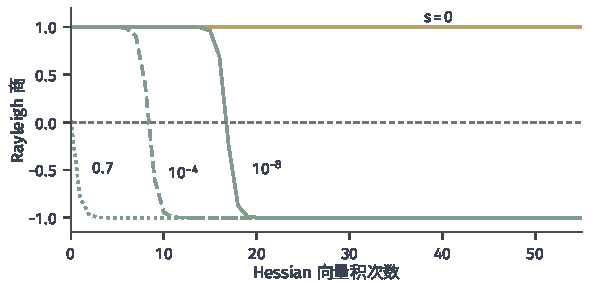
\includegraphics[width=100mm]{figures/05-optimization/02-smooth-optimization/matplotlib/saddle-krylov-blind/figure.pdf}
  \caption{$\bm{H}=\operatorname{diag}(-1,1)$，$L=2$，幂迭代的Rayleigh商随乘积次数的变化，起点是$(s,\sqrt{1-s^2})$。黄线$s=0$永远是$+1$，绿线从左到右$s=0.7,10^{-4},10^{-8}$，拐点依次右移，负曲率最终都被发现。}
  \label{fig:saddle-krylov-blind}
\end{BookInlineFigure}

\paragraph{找到和没有找到，结论不一样}
检测结束有两种结果，它们的可信程度差别很大。若$R^{(k)}\leq-\gamma$，这是一个算出来的事实：$\bm{v}$确实是曲率不超过$-\gamma$的方向，与随机抽样的运气无关。

若没有找到，结论就只能是概率性的。$\bm{v}^{(0)}$可能运气很差，迭代还没转过来就结束了。下面的定理说明，轮数足够多时，这种情况发生的概率很小。图~\ref{fig:saddle-detect-decision}概括了两种结论的区别。

\begin{BookInlineFigure}
  \centering
  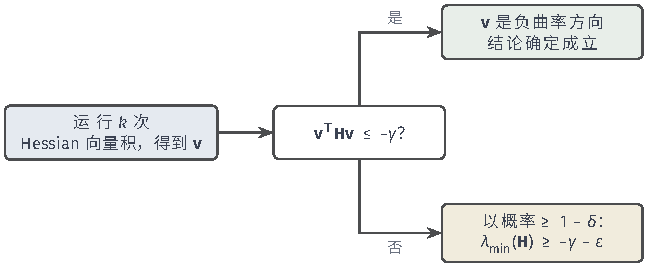
\includegraphics[width=109.6mm]{figures/05-optimization/02-smooth-optimization/tikz/saddle-detect-decision/figure.pdf}
  \caption{负曲率检测的两种结果。使用精确的Hessian向量积时，“找到”给出确定的结论；“未找到”只在随机起点成功的事件上成立，失败概率由$\delta$控制，$\varepsilon$是检测精度。}
  \label{fig:saddle-detect-decision}
\end{BookInlineFigure}

\begin{theorem}[幂迭代的概率保证]
 \label{thm:saddle-power}
 设$\bm{H}\in\mathbb{R}^{n\times n}$对称，$\lVert\bm{H}\rVert_2\leq L$，$\varepsilon\in(0,L]$，$\delta\in(0,1)$。$\bm{v}^{(0)}$在单位球面上均匀分布，幂迭代~\eqref{eq:saddle-power-iteration}运行$k$轮，其中
 \begin{equation}
  k\geq\frac{2L}{\varepsilon}\ln\frac{64Ln}{\pi\varepsilon\delta^3}.
  \label{eq:saddle-power-rounds}
 \end{equation}
 则至少以$1-\delta$的概率，
 \begin{equation}
  \bm{v}^{(k)\top}\bm{H}\bm{v}^{(k)}\leq\lambda_{\min}(\bm{H})+\varepsilon.
  \label{eq:saddle-power-guarantee}
 \end{equation}
\end{theorem}

\begin{proof}
 证明分两步：先说明随机起点在$\bm{q}_1$上的分量不会太小，再说明幂迭代把其余误差压下去。

 第一步处理起点。球面上的均匀分布可以写成$\bm{v}^{(0)}=\bm{z}/\lVert\bm{z}\rVert_2$，其中$\bm{z}$是标准正态向量。由旋转不变性，可以设$c_1=z_1/\lVert\bm{z}\rVert_2$是$\bm{v}^{(0)}$在$\bm{q}_1$上的分量。标准正态密度不超过$1/\sqrt{2\pi}$，所以
 \[
  \mathbb{P}\bigl(\lvert z_1\rvert\leq\tau\bigr)\leq\tau\sqrt{\frac{2}{\pi}}.
 \]

 取$\tau=\tfrac{\delta}{2}\sqrt{\pi/2}$，这个概率不超过$\delta/2$。又因为$\mathbb{E}\lVert\bm{z}\rVert_2^2=n$，由Markov不等式，
 \[
  \mathbb{P}\Bigl(\lVert\bm{z}\rVert_2^2>\frac{2n}{\delta}\Bigr)\leq\frac{\delta}{2}.
 \]

 因此至少以$1-\delta$的概率，两个事件都不发生，此时
 \[
  c_1^2\geq\frac{\tau^2}{2n/\delta}=\frac{\pi\delta^3}{16n}.
 \]

 第二步在这个事件上估计误差。记$a_i=L-\lambda_i$，$a_1$最大且$0\leq a_i\leq2L$；若$a_1=0$，$\bm{H}=L\bm{I}$，结论自动成立，下面设$a_1>0$。$\bm{v}^{(k)}$正比于$\bm{A}^k\bm{v}^{(0)}$，所以由$\bm{v}^\top\bm{H}\bm{v}=L-\bm{v}^\top\bm{A}\bm{v}$，
 \[
  \bm{v}^{(k)\top}\bm{H}\bm{v}^{(k)}-\lambda_{\min}
  =\frac{\sum_ic_i^2a_i^{2k}(a_1-a_i)}{\sum_ic_i^2a_i^{2k}}.
 \]

 把下标分成两组：$a_i\geq a_1-\varepsilon/2$的一组，分子中的因子$a_1-a_i$不超过$\varepsilon/2$，这一组对比值的贡献不超过$\varepsilon/2$。

 其余的下标满足$a_i<a_1-\varepsilon/2$，于是
 \[
  a_i^{2k}\leq a_1^{2k}\Bigl(1-\frac{\varepsilon}{2a_1}\Bigr)^{2k}
  \leq a_1^{2k}\exp\Bigl(-\frac{k\varepsilon}{a_1}\Bigr).
 \]

 分母至少是$c_1^2a_1^{2k}$，$a_1-a_i\leq a_1\leq2L$，$\sum_ic_i^2=1$，$a_1\leq2L$使指数不小于$k\varepsilon/(2L)$。所以这一组的贡献不超过
 \[
  \frac{2L}{c_1^2}\exp\Bigl(-\frac{k\varepsilon}{2L}\Bigr).
 \]

 代入$c_1^2$的下界和条件~\eqref{eq:saddle-power-rounds}，这个量不超过$\varepsilon/2$。两组相加，即得式~\eqref{eq:saddle-power-guarantee}。
\end{proof}

定理中各个量的作用可以逐项核对。$L/\varepsilon$来自幂迭代的收敛速度，要分辨相差$\varepsilon$的特征值，需要的轮数与$L/\varepsilon$成正比。$\ln n$和$\ln(1/\delta)$只出现在对数里，它们是随机起点要付的代价。

结论的含义是：运行满轮数仍然没有发现$R\leq-\gamma$时，以至少$1-\delta$的概率，
\begin{equation}
 \lambda_{\min}(\bm{H})\geq R^{(k)}-\varepsilon>-\gamma-\varepsilon.
 \label{eq:saddle-no-find}
\end{equation}

例中取$L=2$，$n=2$，$\varepsilon=\tfrac14$，$\delta=0.1$，式~\eqref{eq:saddle-power-rounds}要求$k\geq204$。上面的手算只用$2$次乘积就找到了方向。两者不矛盾：定理针对的是任意$\bm{H}$和最坏情形的起点分量，它要保证的是“没有找到”这个结论也能成立。

\paragraph{Lanczos方法}
幂迭代每轮只用最后一个向量，把前面的乘积结果都丢弃了。Lanczos方法保留整个Krylov子空间
\[
 \mathcal{K}_k=\operatorname{span}\bigl\{\bm{v}^{(0)},\bm{H}\bm{v}^{(0)},\ldots,\bm{H}^{k-1}\bm{v}^{(0)}\bigr\},
\]
并在这个子空间上取Rayleigh商的最小值。乘积次数相同，幂迭代的结果也落在同一个子空间内，所以Lanczos给出的值不会更差。它的三项递推和实现细节可参考\BookChapterRef{chap:krylov-methods}{卷二第15章“Krylov子空间法”}，这里只用它的结果：标准正交基下$\bm{H}$的投影是三对角矩阵$\bm{T}_k$，$\bm{T}_k$的最小特征值就是这个子空间上的最小Rayleigh商。

下面用一个三阶矩阵比较两者，它是在例子的Hessian上补一个中间特征值得到的：
\[
 \bm{H}=\operatorname{diag}(-1,1,2),\qquad
 \bm{v}^{(0)}=\frac{1}{\sqrt3}(1,1,1)^\top.
\]

第一步的对角元和残差是
\[
 \alpha_1=\frac23,\qquad
 \bm{w}=\bm{H}\bm{v}^{(0)}-\alpha_1\bm{v}^{(0)}
 =\frac{1}{3\sqrt3}\begin{bmatrix}-5\\1\\4\end{bmatrix},\qquad
 \beta_1=\lVert\bm{w}\rVert_2=\frac{\sqrt{14}}{3}.
\]

第二个基向量是$\bm{w}/\beta_1$，由此计算第二个对角元，得到
\[
 \alpha_2=\frac{-25+1+32}{42}=\frac{4}{21},\qquad
 \bm{T}_2=\begin{bmatrix}2/3&\sqrt{14}/3\\\sqrt{14}/3&4/21\end{bmatrix}.
\]

$\bm{T}_2$的最小特征值约为$-0.841$。同样用$2$次乘积，$L=2$的幂迭代$\bm{v}^{(1)}\propto(3,1,0)$给出$-0.8$。差距在小矩阵上不明显，在谱分布更不利时就很大了。

图~\ref{fig:saddle-power-lanczos}是一个$n=400$的例子。第二小的特征值紧贴最小特征值时，幂迭代几乎停滞，Lanczos仍然很快。原因是$k$次乘积相当于选一个$k$次多项式去放大$\bm{q}_1$分量，幂迭代固定用$a^k$，Lanczos等于在所有$k$次多项式中选最好的一个。

\begin{BookInlineFigure}
  \centering
  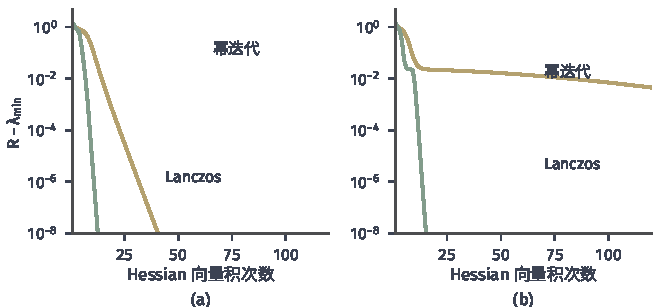
\includegraphics[width=112mm]{figures/05-optimization/02-smooth-optimization/matplotlib/saddle-power-lanczos/figure.pdf}
  \caption{同一个随机起点下幂迭代（黄，$L=2$）与Lanczos方法（绿）的Rayleigh商误差，$n=400$，$\lambda_{\min}=-0.2$，其余特征值在$[0.5,2]$上均匀取样，只有第二小的特征值另行指定。(a)第二小特征值为$0.3$。(b)第二小特征值为$-0.17$，与最小特征值很接近。}
  \label{fig:saddle-power-lanczos}
\end{BookInlineFigure}

定量结果是：均匀随机起点的Lanczos方法运行约$\sqrt{L/\varepsilon}\,\ln(n/\delta^2)$次乘积，就以至少$1-\delta$的概率达到精度$\varepsilon$。与定理~\ref{thm:saddle-power}相比，$L/\varepsilon$换成了它的平方根。证明需要用到Chebyshev多项式在区间外的增长估计，篇幅较长，读者可查阅数值线性代数的专门著作，这里只把它作为不加证明的事实使用。

Lanczos的计算也有代价：要存基向量才能算出方向，三项递推在有限精度下会失去正交性，运行次数多时需要重新正交化或重启。

\paragraph{误差怎样记入}
前面的结论默认Hessian向量积是精确的，用差分时要补上式~\eqref{eq:saddle-hvp-error}。对“找到”这一方，算出的$\hat{R}=\bm{v}^\top\hat{\bm{u}}$与真实Rayleigh商至多相差$Mh/2$，把判定条件改成$\hat{R}\leq-\gamma-Mh/2$，就能确定地推出$R(\bm{v})\leq-\gamma$。

对“没有找到”这一方，差分误差还会改变迭代本身，定理~\ref{thm:saddle-power}不能直接套用，分析时必须把每一轮的乘积误差累加进去。实际程序里，要做这一判断时通常用自动微分得到精确的乘积。表~\ref{tab:saddle-detect-compare}总结了几种方式。

\begin{BookInlineTable}
  \centering
  \begin{tabular}{@{}llll@{}}
    \toprule
    检测方式 & 成本 & 找到时 & 未找到时\\
    \midrule
    特征分解 & $O(n^3)$ & 确定 & 确定\\
    Cholesky试探 & $O(n^3)$，只判断 & 确定 & 确定\\
    幂迭代 & $O(\frac{L}{\varepsilon}\ln\frac{n}{\delta})$次乘积 & 确定 & $\geq1-\delta$\\
    Lanczos & $O(\sqrt{\frac{L}{\varepsilon}}\ln\frac{n}{\delta})$次乘积 & 确定 & $\geq1-\delta$\\
    差分乘积 & 每次两个梯度 & 加余量$Mh/2$ & 累加误差\\
    \bottomrule
  \end{tabular}
  \caption{负曲率检测方式的比较，“确定”不计舍入误差，“$\geq1-\delta$”指结论成立的概率。$O(\cdot)$中省略了$L/\varepsilon$的对数因子。}
  \label{tab:saddle-detect-compare}
\end{BookInlineTable}


\section{离开鞍点}
\label{sec:saddle-escape}

迭代点已经到了梯度很小的鞍点邻域，怎样离开？回答取决于手里有什么信息。知道一个负曲率方向时，可以沿它走一步；只有梯度时，可以给迭代点一点随机扰动，让梯度下降自己放大不稳定的分量；有二次模型时，可以保留模型的不定性，让子问题自己走到负曲率的一侧。三种机制各有条件，都不能把严格鞍点的结论直接搬到退化驻点上。

\subsection{负曲率步}
\label{sec:saddle-nc-step}

上一节的检测给出了单位向量$\bm{v}$，满足$\bm{v}^\top\bm{H}\bm{v}\leq-\gamma$。站在山口上，这是一条明确的下坡路。问题是这样走一步能保证下降多少，步长又该取多大。

\paragraph{为什么要控制Hessian的变化}
二阶模型沿$\bm{v}$的预测是$-\tfrac12\gamma\alpha^2$，步长越大下降越多，但这个预测不可能一直成立。模型只在局部有效，走远了Hessian会变。例中沿$x_1$轴，
\[
 f(\alpha,0)=\frac14\bigl(\alpha^2-1\bigr)^2.
\]

$\alpha=1$处到达谷底，$\alpha=\sqrt2$处函数值回到$1/4$，再往前目标反而高于起点。所以负曲率方向不能无限延长，步长要受Hessian变化速度的约束，这个速度就是$M$。下面的引理给出二阶模型的误差。

\begin{lemma}[三次上界]
 \label{lem:saddle-cubic}
 设$\nabla^2f$在凸集$\bm{U}$上是$M$-Lipschitz的，$\bm{x}$与$\bm{x}+\bm{p}$都在$\bm{U}$中。记$\bm{g}=\nabla f(\bm{x})$，$\bm{H}=\nabla^2f(\bm{x})$，则
 \begin{equation}
  \Bigl\lvert f(\bm{x}+\bm{p})-f(\bm{x})-\langle\bm{g},\bm{p}\rangle-\frac12\bm{p}^\top\bm{H}\bm{p}\Bigr\rvert
  \leq\frac{M}{6}\lVert\bm{p}\rVert_2^3.
  \label{eq:saddle-cubic}
 \end{equation}
\end{lemma}

\begin{proof}
 令$\phi(s)=f(\bm{x}+s\bm{p})$，$s\in[0,1]$。由积分余项形式的Taylor公式，
 \[
  \phi(1)=\phi(0)+\phi'(0)+\int_0^1(1-s)\phi''(s)\,\mathrm{d}s.
 \]

 其中$\phi'(0)=\langle\bm{g},\bm{p}\rangle$。又因为$\int_0^1(1-s)\,\mathrm{d}s=\tfrac12$，二次项可以写进同一个积分，得到
 \[
  f(\bm{x}+\bm{p})-f(\bm{x})-\langle\bm{g},\bm{p}\rangle-\frac12\bm{p}^\top\bm{H}\bm{p}
  =\int_0^1(1-s)\bigl(\phi''(s)-\phi''(0)\bigr)\,\mathrm{d}s.
 \]

 $\phi$的二阶导数是Hessian沿$\bm{p}$的二次型，由Lipschitz条件，
 \[
  \lvert\phi''(s)-\phi''(0)\rvert
  =\bigl\lvert\bm{p}^\top\bigl(\nabla^2f(\bm{x}+s\bm{p})-\bm{H}\bigr)\bm{p}\bigr\rvert
  \leq Ms\lVert\bm{p}\rVert_2^3.
 \]

 代入并用$\int_0^1(1-s)s\,\mathrm{d}s=\tfrac16$，即得式~\eqref{eq:saddle-cubic}。
\end{proof}

\paragraph{选符号，定步长}
梯度不为零时，$\bm{v}$和$-\bm{v}$的曲率相同，一阶项却相反。所以先选符号，使一阶项不起反作用。下面的定理给出一步的下降量。

\begin{theorem}[负曲率步的下降]
 \label{thm:saddle-nc-step}
 设单位向量$\bm{v}$满足$\bm{v}^\top\bm{H}\bm{v}\leq-\gamma<0$和$\langle\bm{g},\bm{v}\rangle\leq0$，引理~\ref{lem:saddle-cubic}的条件对$\bm{p}=\alpha\bm{v}$成立。则对$\alpha>0$，
 \begin{equation}
  f(\bm{x}+\alpha\bm{v})\leq f(\bm{x})-\frac{\gamma}{2}\alpha^2+\frac{M}{6}\alpha^3.
  \label{eq:saddle-nc-bound}
 \end{equation}
 取$\alpha=2\gamma/M$时，
 \begin{equation}
  f(\bm{x}+\alpha\bm{v})\leq f(\bm{x})-\frac{2\gamma^3}{3M^2}.
  \label{eq:saddle-nc-decrease}
 \end{equation}
\end{theorem}

\begin{proof}
 由式~\eqref{eq:saddle-cubic}取$\bm{p}=\alpha\bm{v}$，$\lVert\bm{p}\rVert_2=\alpha$，得到
 \[
  f(\bm{x}+\alpha\bm{v})\leq f(\bm{x})+\alpha\langle\bm{g},\bm{v}\rangle+\frac{\alpha^2}{2}\bm{v}^\top\bm{H}\bm{v}+\frac{M}{6}\alpha^3.
 \]

 由$\langle\bm{g},\bm{v}\rangle\leq0$和$\bm{v}^\top\bm{H}\bm{v}\leq-\gamma$，即得式~\eqref{eq:saddle-nc-bound}。右端作为$\alpha$的函数，对$\alpha$求导得$-\gamma\alpha+\tfrac12M\alpha^2$，在$\alpha=2\gamma/M$处取到最小。代入得
 \[
  -\frac{\gamma}{2}\cdot\frac{4\gamma^2}{M^2}+\frac{M}{6}\cdot\frac{8\gamma^3}{M^3}
  =-\frac{2\gamma^3}{M^2}+\frac{4\gamma^3}{3M^2}
  =-\frac{2\gamma^3}{3M^2}.
 \]
\end{proof}

下降量只依赖负曲率的大小和Hessian的变化速度，与梯度多小无关。这正是它补上梯度步短板的地方：梯度步的保证是$\lVert\bm{g}\rVert_2^2/(2L)$，鞍点附近这个量几乎为零。

例中在原点取$\bm{v}=(1,0)$，$\gamma=1$，$M=6$，步长$\alpha=1/3$。定理保证的下降是
\[
 \frac{2\gamma^3}{3M^2}=\frac{1}{54}\approx0.0185.
\]
实际下降是
\[
 f(\bm{0})-f\bigl(\tfrac13,0\bigr)=\frac14-\frac{16}{81}\approx0.0525.
\]
图~\ref{fig:saddle-nc-slice}(a)沿$x_1$轴比较目标（蓝）、二次模型（绿）和三次上界（紫）。三次上界在$\bm{U}$内从上方盖住目标，绿点$\alpha=1/3$是上界的最低点，这个步长比实际的最好步长$\alpha=1$保守得多。

\begin{BookInlineFigure}
  \centering
  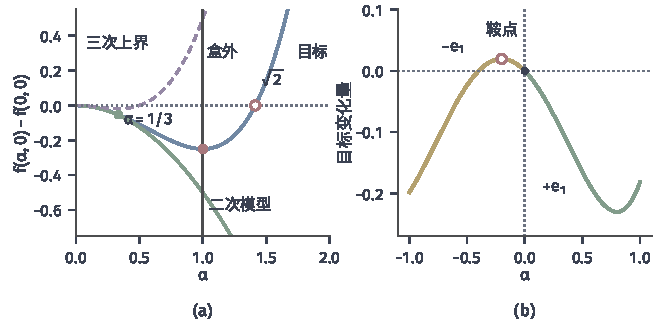
\includegraphics[width=112mm]{figures/05-optimization/02-smooth-optimization/matplotlib/saddle-nc-slice/figure.pdf}
  \caption{沿负曲率方向的一维截面。(a)原点沿$\bm{e}_1$：蓝线是目标减去$f(\bm{0})$，绿线是二次模型$-\alpha^2/2$，紫色虚线是三次上界$-\alpha^2/2+\alpha^3$，竖线是带形$\bm{U}$的边界。空心点$\alpha=\sqrt2$处目标回到起点的值。(b)从$(0.2,0)$出发沿$\pm\bm{e}_1$的目标变化，此处$\langle\bm{g},\bm{e}_1\rangle<0$。绿线一开始就下降，黄线先升到鞍点的高度才下降。}
  \label{fig:saddle-nc-slice}
\end{BookInlineFigure}

符号的作用见图~\ref{fig:saddle-nc-slice}(b)。在$(0.2,0)$处，梯度的第一个分量是$0.008-0.2=-0.192$，$+\bm{e}_1$满足$\langle\bm{g},\bm{v}\rangle<0$。朝$-\bm{e}_1$走，目标要先爬回鞍点才开始下降，一阶项抵消了曲率的好处。

\paragraph{不知道$M$时}
步长$2\gamma/M$要用到$M$，多数问题不知道它的值。这时可以回溯：从$\alpha_0$开始，不断折半，直到满足
\begin{equation}
 f(\bm{x}+\alpha\bm{v})\leq f(\bm{x})-\frac{\gamma}{4}\alpha^2.
 \label{eq:saddle-nc-backtrack}
\end{equation}

由式~\eqref{eq:saddle-nc-bound}，条件成立只需要
\[
 -\frac12\gamma\alpha^2+\frac16M\alpha^3\leq-\frac14\gamma\alpha^2,
\]
也就是$\alpha\leq3\gamma/(2M)$。折半回溯接受的步长因此不小于$\min\{\alpha_0,3\gamma/(4M)\}$，当$\alpha_0$足够大时，一步的下降不少于
\[
 \frac{\gamma}{4}\Bigl(\frac{3\gamma}{4M}\Bigr)^2=\frac{9\gamma^3}{64M^2}.
\]
例中取$\alpha_0=2$，$f(2,0)=9/4$被拒绝，$\alpha=1$时$f(1,0)=0\leq\tfrac14-\tfrac14$，被接受，一步到达谷底。

\paragraph{主要思想：梯度步和负曲率步交替}
梯度步在梯度大时有效，负曲率步在梯度小时仍然有效，两者正好互补。算法每轮先看梯度：梯度大就走梯度步；梯度小才花力气检测负曲率；两者都不能下降就停止。写成公式，
\begin{equation}
 \bm{x}^{(t+1)}=
 \begin{cases}
  \bm{x}^{(t)}-\dfrac{1}{L}\bm{g}^{(t)}, & \lVert\bm{g}^{(t)}\rVert_2>\varepsilon_g,\\
  \bm{x}^{(t)}+\dfrac{2\gamma^{(t)}}{M}\bm{v}^{(t)}, & \text{其他情形且检测到负曲率}.
 \end{cases}
 \label{eq:saddle-nc-update}
\end{equation}
其中单位向量$\bm{v}^{(t)}$的曲率是$-\gamma^{(t)}$，符号已经选定。$\varepsilon_g$和$\varepsilon_H$是梯度和曲率的容差，第~\ref{sec:saddle-stopping}节再讨论怎样取值。

\needspace{6\baselineskip}
\paragraph{变量}
算法要维护的量是：
\begin{itemize}
 \item $\bm{x}^{(t)}\in\mathbb{R}^n$：当前点；
 \item $\bm{g}^{(t)}\in\mathbb{R}^n$：当前梯度，每轮读取一次；
 \item $\bm{v}^{(t)}\in\mathbb{R}^n$，$\gamma^{(t)}>0$：只在梯度小的轮次计算的负曲率方向及其大小。
\end{itemize}

\paragraph{初始化}
选定$\bm{x}^{(0)}$、$L$、$M$和容差。例中$L=2$，$M=6$，$\varepsilon_g=0.1$，$\varepsilon_H=\sqrt{M\varepsilon_g}\approx0.775$，起点取在$x_2$轴上，并且用特征分解做检测：
\[
 \bm{x}^{(0)}=\begin{bmatrix}0\\1\end{bmatrix}.
\]

\paragraph{每轮更新}
第$t$轮依次执行以下步骤，直到第$3$步宣布停止。

\begin{enumerate}
 \item 计算$\bm{g}^{(t)}$。若$\lVert\bm{g}^{(t)}\rVert_2>\varepsilon_g$，由式~\eqref{eq:saddle-nc-update}走梯度步，进入下一轮。例中前$4$轮$x_1$一直是$0$，$x_2$每轮减半：
 \[
  \bm{x}^{(1)}=\begin{bmatrix}0\\0.5\end{bmatrix},\quad
  \bm{x}^{(2)}=\begin{bmatrix}0\\0.25\end{bmatrix},\quad
  \bm{x}^{(3)}=\begin{bmatrix}0\\0.125\end{bmatrix},\quad
  \bm{x}^{(4)}=\begin{bmatrix}0\\0.0625\end{bmatrix}.
 \]
 \item 否则检测负曲率。例中第$4$轮$\lVert\bm{g}^{(4)}\rVert_2=0.0625\leq0.1$，由式~\eqref{eq:saddle-example-derivatives}，
 \[
  \bm{H}^{(4)}=\operatorname{diag}(-1,1),\qquad\lambda_{\min}=-1<-\varepsilon_H.
 \]
 \item 若$\lambda_{\min}\geq-\varepsilon_H$，停止并返回$\bm{x}^{(t)}$。否则取$\bm{v}^{(t)}$为最小特征向量，$\gamma^{(t)}=-\lambda_{\min}$，选好符号，由式~\eqref{eq:saddle-nc-update}走负曲率步。例中第$4$轮$\langle\bm{g}^{(4)},\bm{e}_1\rangle=0$，取$\bm{v}=\bm{e}_1$，步长$1/3$，得到
 \[
  \bm{x}^{(5)}=\begin{bmatrix}1/3\\0.0625\end{bmatrix}.
 \]
\end{enumerate}

此后梯度已经变大，算法回到梯度步。表~\ref{tab:saddle-nc-run}列出全过程。第$9$轮$\lVert\bm{g}^{(9)}\rVert_2=0.060\leq0.1$，Hessian是$\operatorname{diag}(1.815,1)$，$\lambda_{\min}=1\geq-\varepsilon_H$，算法停止，最终得到$\bm{x}^{(9)}\approx(0.9686,0.0039)$。

\begin{BookInlineTable}
  \centering
  \begin{tabular}{@{}rccccl@{}}
    \toprule
    $t$ & $\bm{x}^{(t)}$ & $f$ & $\lVert\bm{g}^{(t)}\rVert_2$ & $\lambda_{\min}$ & 本轮动作\\
    \midrule
    $0$ & $(0,\ 1)$ & $0.7500$ & $1.000$ & $-1$ & 梯度步\\
    $1$ & $(0,\ 0.5)$ & $0.3750$ & $0.500$ & $-1$ & 梯度步\\
    $2$ & $(0,\ 0.25)$ & $0.2813$ & $0.250$ & $-1$ & 梯度步\\
    $3$ & $(0,\ 0.125)$ & $0.2578$ & $0.125$ & $-1$ & 梯度步\\
    $4$ & $(0,\ 0.0625)$ & $0.2520$ & $0.063$ & $-1$ & 负曲率步\\
    $5$ & $(0.3333,\ 0.0625)$ & $0.1995$ & $0.303$ & $-0.667$ & 梯度步\\
    $6$ & $(0.4815,\ 0.0313)$ & $0.1480$ & $0.371$ & $-0.305$ & 梯度步\\
    $7$ & $(0.6664,\ 0.0156)$ & $0.0774$ & $0.371$ & $0.332$ & 梯度步\\
    $8$ & $(0.8516,\ 0.0078)$ & $0.0189$ & $0.234$ & $1$ & 梯度步\\
    $9$ & $(0.9686,\ 0.0039)$ & $0.0010$ & $0.060$ & $1$ & 停止\\
    \bottomrule
  \end{tabular}
  \caption{梯度步与负曲率步在目标~\eqref{eq:saddle-example}上的运行。$\varepsilon_g=0.1$，$\varepsilon_H\approx0.775$，$\lambda_{\min}$是Hessian~\eqref{eq:saddle-example-derivatives}的最小特征值，第$8$、$9$轮第一个对角元已大于$1$，最小特征值取到$1$。}
  \label{tab:saddle-nc-run}
\end{BookInlineTable}

图~\ref{fig:saddle-nc-run}对照了不做检测的梯度下降。两者前$4$轮完全相同；梯度下降从此沿$x_2$轴收敛到鞍点，目标停在$1/4$，而负曲率步使迭代点离开了这条轴。

\begin{BookInlineFigure}
  \centering
  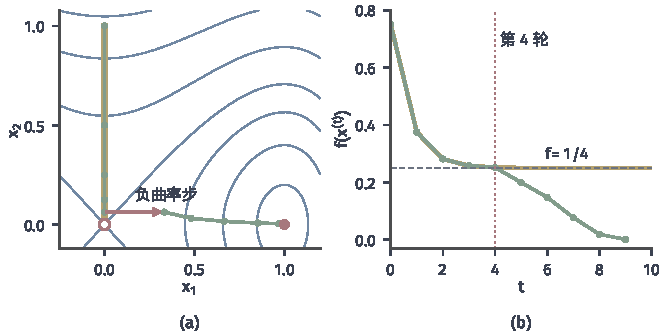
\includegraphics[width=112mm]{figures/05-optimization/02-smooth-optimization/matplotlib/saddle-nc-run/figure.pdf}
  \caption{从$(0,1)$出发的运行，步长$\alpha=1/2$。(a)绿色折线是梯度步与负曲率步的路径，红色箭头是第$4$轮的负曲率步，黄线（被绿线部分遮挡）是梯度下降，沿$x_2$轴收敛到空心点所示的鞍点。(b)目标值随轮数的变化，黄线趋于虚线$f=1/4$，绿线在红色点线所示的第$4$轮之后继续下降。}
  \label{fig:saddle-nc-run}
\end{BookInlineFigure}

\paragraph{算法分析}
每轮的下降都有下界，累加就得到轮数上界，论证与第~\ref{chap:smooth-foundations}章的累加下降相同。下面的定理把检测精度写成一个参数，以便同时覆盖精确和近似检测。

\begin{theorem}[交替算法的轮数]
 \label{thm:saddle-nc-count}
 设$f$有下界$f_{\inf}$，$\nabla f$和$\nabla^2f$在包含各步线段的凸集上分别是$L$-Lipschitz和$M$-Lipschitz的。设每次走负曲率步时都有$\gamma^{(t)}\geq\gamma_0>0$，记$\Delta_f=f(\bm{x}^{(0)})-f_{\inf}$。则算法~\eqref{eq:saddle-nc-update}停止之前的轮数$T$满足
 \begin{equation}
  T\leq\Delta_f\max\Bigl\{\frac{2L}{\varepsilon_g^2},\ \frac{3M^2}{2\gamma_0^3}\Bigr\}.
  \label{eq:saddle-nc-count}
 \end{equation}
\end{theorem}

\begin{proof}
 由下降引理，走梯度步的轮次下降至少$\lVert\bm{g}^{(t)}\rVert_2^2/(2L)$，而这些轮次$\lVert\bm{g}^{(t)}\rVert_2>\varepsilon_g$，下降超过$\varepsilon_g^2/(2L)$。

 由定理~\ref{thm:saddle-nc-step}，走负曲率步的轮次下降至少$2\gamma_0^3/(3M^2)$。记两者中较小的为$c$，累加$T$轮得
 \[
  \Delta_f\geq f(\bm{x}^{(0)})-f(\bm{x}^{(T)})\geq Tc.
 \]
 除以$c$即得式~\eqref{eq:saddle-nc-count}。
\end{proof}

例中$\Delta_f=3/4$。精确检测对应$\gamma_0=\varepsilon_H$，两项分别是$400$和约$116$，上界是$300$轮，实际只用了$9$轮。这也是一个最坏情形的界，它只用到$L$、$M$、$\Delta_f$，没有用到例子的具体形状。

\paragraph{适用范围}
这个算法要求能算出负曲率方向，在第~\ref{sec:saddle-detection}节的意义下，检测是确定的或者带失败概率的，第~\ref{sec:saddle-stopping}节再把这部分成本计入。定理只保证算法在有限步内停止，停止时的点满足两个容差，它不说明这个点是局部极小点。Hessian不是Lipschitz连续时，式~\eqref{eq:saddle-cubic}没有依据，步长公式也就失去了基础。

\subsection{扰动梯度法}
\label{sec:saddle-perturbed}

现在假设只能读取梯度，连Hessian向量积也不用。梯度下降在鞍点附近究竟怎样运动，是分析的起点。

\paragraph{鞍点附近的线性运动}
设$\bm{x}^\star$是严格鞍点，$\bm{H}=\nabla^2f(\bm{x}^\star)$。在$\bm{x}^\star$附近$\nabla f(\bm{x})\approx\bm{H}(\bm{x}-\bm{x}^\star)$，梯度下降近似于线性迭代：
\begin{equation}
 \bm{x}^{(t+1)}-\bm{x}^\star\approx(\bm{I}-\alpha\bm{H})\bigl(\bm{x}^{(t)}-\bm{x}^\star\bigr).
 \label{eq:saddle-linear}
\end{equation}

沿特征向量$\bm{q}_i$的分量每步乘以$1-\alpha\lambda_i$。$\alpha=1/L$时，正曲率方向的因子在$[0,1)$内，分量收缩；负曲率方向的因子$1+\alpha\lvert\lambda_i\rvert$大于$1$，分量放大。这正是第~\ref{sec:saddle-detection}节的幂迭代：梯度下降本身就在放大最负的方向。

例中两个坐标的迭代是
\[
 x_1^{(t+1)}=\frac32x_1^{(t)}-\frac12\bigl(x_1^{(t)}\bigr)^3,\qquad
 x_2^{(t+1)}=\frac12x_2^{(t)}.
\]
在原点附近，$x_1$每步约乘以$1.5$，$x_2$每步乘以$0.5$。图~\ref{fig:saddle-gd-linear}(b)的对数坐标下，两者都是直线，直到$x_1$接近$1$才不再增长。

\begin{BookInlineFigure}
  \centering
  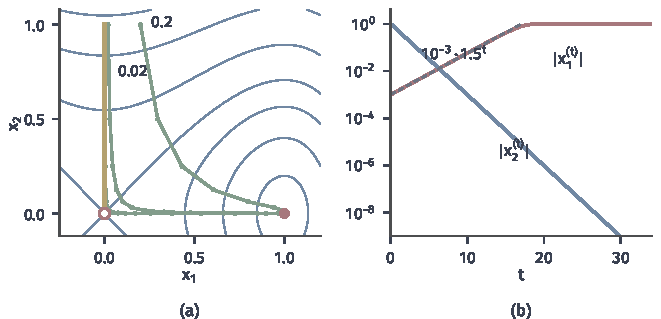
\includegraphics[width=112mm]{figures/05-optimization/02-smooth-optimization/matplotlib/saddle-gd-linear/figure.pdf}
  \caption{目标~\eqref{eq:saddle-example}上步长$1/2$的梯度下降。(a)从$(s,1)$出发的路径，绿线$s=0.2,0.02,0.002$，黄线$s=0$沿$x_2$轴收敛到鞍点。$s$越小，路径越贴近鞍点，徘徊越久。(b)从$(10^{-3},1)$出发，$\lvert x_1^{(t)}\rvert$（红）按$1.5^t$增长（灰色虚线），$\lvert x_2^{(t)}\rvert$（蓝）按$0.5^t$衰减。}
  \label{fig:saddle-gd-linear}
\end{BookInlineFigure}

\paragraph{什么样的初值会收敛到鞍点}
例中只要$x_1^{(0)}\neq0$，这个分量迟早被放大；只有$x_1^{(0)}=0$的点才一直留在$x_2$轴上，收敛到鞍点。这条轴是鞍点的\term{稳定流形}（stable manifold），二维平面上它的面积为零。

这个观察有严格的版本：设$f$二阶连续可微，$\nabla f$全局$L$-Lipschitz，步长$0<\alpha<1/L$，初值的分布对Lebesgue测度绝对连续，则梯度下降收敛到严格鞍点的概率为零\scite{lee2016gradient}。证明需要把迭代写成微分同胚，再用中心稳定流形定理，篇幅较长，读者可查阅原文。

这个结论有三个限度。第一，它的随机性只来自初值，之后的迭代完全确定。第二，它只排除收敛到严格鞍点，不说明会收敛到局部极小点，迭代也可能根本不收敛。第三，它是渐近的，没有说需要多少步。第三点不能靠更细的分析补上：要让$\lvert x_1\rvert$增长到$0.5$，例中的轮数如下。

\begin{BookInlineTable}
  \centering
  \begin{tabular}{@{}ccccc@{}}
    \toprule
    $x_1^{(0)}$ & $10^{-3}$ & $10^{-6}$ & $10^{-9}$ & $10^{-12}$\\
    \midrule
    轮数 & $16$ & $33$ & $50$ & $67$\\
    \bottomrule
  \end{tabular}
  \caption{目标~\eqref{eq:saddle-example}上$\lvert x_1^{(t)}\rvert$首次达到$0.5$所需的轮数。}
  \label{tab:saddle-escape-time}
\end{BookInlineTable}

初值的$x_1$可以任意接近零，轮数就可以任意大。所以普通梯度下降没有一个对所有初值都成立的有限步上界。要得到有限步的保证，必须让算法自己把迭代点推离稳定流形。

\paragraph{主要思想：只需要一点扰动}
图~\ref{fig:saddle-stuck-band}用数值实验看这件事。以原点为中心取半径$0.25$的圆盘，把每个点作为初值运行若干步梯度下降，再标出目标没有下降足够多的初值。这些“卡住”的初值组成一条沿$x_2$方向的窄带，步数越多，窄带越窄。

\begin{BookInlineFigure}
  \centering
  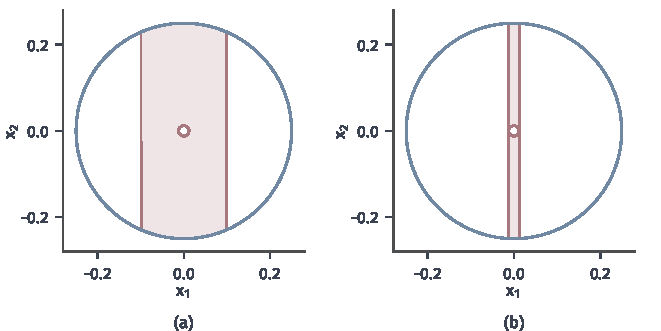
\includegraphics[width=112mm]{figures/05-optimization/02-smooth-optimization/matplotlib/saddle-stuck-band/figure.pdf}
  \caption{从半径$0.25$的圆盘（蓝线）内出发的梯度下降，步长$1/2$。红色窄带内的初值在$T$步后仍有$f>1/4-0.05$。(a)$T=3$，带的半宽约$0.099$。(b)$T=8$，带的半宽约$0.013$。窄带以外的点都已离开鞍点。}
  \label{fig:saddle-stuck-band}
\end{BookInlineFigure}

因此，在鞍点附近的小球内随机选一个点，落在窄带里的概率很小。图~\ref{fig:saddle-perturb-band}是概率的几何含义：窄带的体积与整个球的体积之比。只要球内的点几乎都能离开，加一点随机扰动就够了，扰动不需要很大。

\begin{BookInlineFigure}
  \centering
  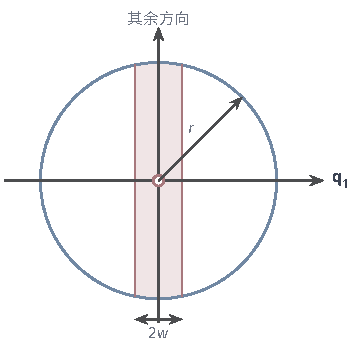
\includegraphics[width=61mm]{figures/05-optimization/02-smooth-optimization/tikz/saddle-perturb-band/figure.pdf}
  \caption{半径$r$的球内，沿$\bm{q}_1$方向半宽$w$的窄带。均匀随机的扰动落入窄带的概率就是两者的体积比。窄带外的点在$\bm{q}_1$上的分量至少是$w$。}
  \label{fig:saddle-perturb-band}
\end{BookInlineFigure}

先在二次目标上把这件事算清楚，此时$\bm{x}^\star$处的线性近似~\eqref{eq:saddle-linear}是精确的，全部论证都能写出来。

\begin{theorem}[二次目标上的逃离]
 \label{thm:saddle-quadratic-escape}
 设$f(\bm{x})=\tfrac12\bm{x}^\top\bm{H}\bm{x}$，$\bm{H}\in\mathbb{R}^{n\times n}$对称，$\lVert\bm{H}\rVert_2\leq L$，$\lambda_{\min}(\bm{H})=-\gamma<0$。$\bm{x}^{(0)}$在半径$r$的球内均匀分布，按步长$1/L$作梯度下降，迭代矩阵是$\bm{I}-\bm{H}/L$。给定$F>0$，$\delta\in(0,1)$，若
 \begin{equation}
  T\geq\frac{L}{\gamma}\ln\frac{4n\,(Lr^2+2F)}{\pi\gamma\,\delta^2r^2},
  \label{eq:saddle-quadratic-steps}
 \end{equation}
 则至少以$1-\delta$的概率，
 \begin{equation}
  f(\bm{x}^{(T)})\leq-F.
  \label{eq:saddle-quadratic-result}
 \end{equation}
\end{theorem}

\begin{proof}
 设$c_i=\langle\bm{x}^{(0)},\bm{q}_i\rangle$，$\bm{q}_1$对应$-\gamma$。证明分三步。

 第一步估计$c_1$不太小的概率。令$w>0$，事件$\lvert c_1\rvert\leq w$是球内半宽$w$的窄带，它的体积不超过宽度$2w$乘以$(n-1)$维截面的最大体积。记$V_m$为$m$维单位球的体积，于是
 \[
  \mathbb{P}\bigl(\lvert c_1\rvert\leq w\bigr)\leq\frac{2w\,r^{n-1}V_{n-1}}{r^nV_n}=\frac{2w}{r}\cdot\frac{V_{n-1}}{V_n}.
 \]

 单位球体积比由Gamma函数给出，再用Wendel不等式$\Gamma(x+\tfrac12)/\Gamma(x)\leq\sqrt{x}$，取$x=\tfrac{n+1}{2}$，得到
 \[
  \frac{V_{n-1}}{V_n}=\frac{\Gamma(\frac n2+1)}{\sqrt\pi\,\Gamma(\frac{n+1}{2})}\leq\sqrt{\frac{n+1}{2\pi}}\leq\sqrt{\frac{n}{\pi}}.
 \]

 取$w=\tfrac{r\delta}{2}\sqrt{\pi/n}$，窄带的概率不超过$\delta$。所以至少以$1-\delta$的概率，
 \[
  c_1^2\geq w^2=\frac{\pi\delta^2r^2}{4n}.
 \]

 第二步写出迭代的目标值。$\bm{x}^{(T)}$在$\bm{q}_i$上的分量是$(1-\lambda_i/L)^Tc_i$，所以
 \[
  f(\bm{x}^{(T)})=\frac12\sum_i\lambda_i\Bigl(1-\frac{\lambda_i}{L}\Bigr)^{2T}c_i^2.
 \]

 对$\lambda_i\geq0$的项，$0\leq1-\lambda_i/L\leq1$，这些项的和不超过$\tfrac12L\sum_ic_i^2\leq\tfrac12Lr^2$。对$\lambda_i<0$的项，它们都不大于零，只保留$\bm{q}_1$这一项，得到
 \[
  f(\bm{x}^{(T)})\leq\frac12Lr^2-\frac12\gamma\Bigl(1+\frac{\gamma}{L}\Bigr)^{2T}c_1^2.
 \]

 第三步确定步数。要使右端不超过$-F$，只需
 \[
  \Bigl(1+\frac{\gamma}{L}\Bigr)^{2T}\geq\frac{Lr^2+2F}{\gamma c_1^2}.
 \]

 由$\gamma\leq L$和不等式$\ln(1+y)\geq y/2$（$0\leq y\leq1$），左端的对数至少是$T\gamma/L$。代入$c_1^2$的下界，条件~\eqref{eq:saddle-quadratic-steps}恰好保证上式成立。
\end{proof}

定理把扰动的作用说清楚了。步数的主要部分是$L/\gamma$，即放大一倍需要的步数。维数$n$和失败概率$\delta$都在对数里，这是因为分量按指数增长，初值小一个倍数只增加常数步。高维时随机向量在任一方向上的分量约为$r/\sqrt n$，这个$\sqrt n$只通过$\ln n$进入步数。

例中在二次近似$\operatorname{diag}(-1,1)$上取$n=2$，$L=2$，$\gamma=1$，$r=0.05$，$F=0.05$，$\delta=0.1$，式~\eqref{eq:saddle-quadratic-steps}的右端约为$18.6$，所以$T=19$就够了。

图~\ref{fig:saddle-escape-scaling}用模拟检验定理。Hessian取$\operatorname{diag}(-\gamma,1,\ldots,1)$，其余参数同上，统计达到$f\leq-F$的步数。(a)中维数从$2$增加到$10^5$，中位数只从$7$增加到$20$。(b)中步数随$\gamma$减小按$1/\gamma$增长。上界比实际步数略大，但两种依赖关系都吻合。

\begin{BookInlineFigure}
  \centering
  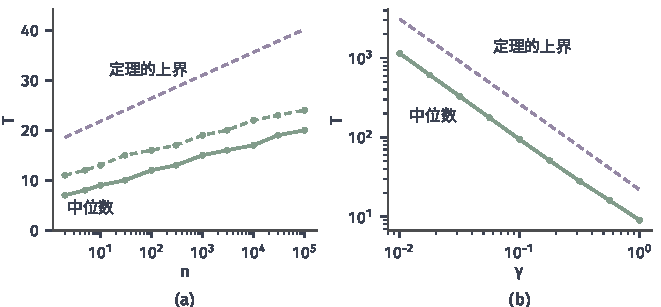
\includegraphics[width=112mm]{figures/05-optimization/02-smooth-optimization/matplotlib/saddle-escape-scaling/figure.pdf}
  \caption{二次目标上达到$f\leq-F$所需步数的模拟，每组$3000$次，$L=2$，$r=0.05$，$F=0.05$，Hessian取$\operatorname{diag}(-\gamma,1,\ldots,1)$。绿色实线是中位数，绿色虚线是$90\%$分位数，紫色虚线是式~\eqref{eq:saddle-quadratic-steps}在$\delta=0.1$时的上界。(a)$\gamma=1$，步数随维数$n$对数增长。(b)$n=10$，步数约与$1/\gamma$成正比。}
  \label{fig:saddle-escape-scaling}
\end{BookInlineFigure}

把上面的想法组成算法就是\term{扰动梯度法}（perturbed gradient method）：平时走梯度步；梯度小时加一次随机扰动，再运行一段固定长度的梯度步作为检验。目标下降了足够多，说明确实离开了鞍点，继续；否则就认为这里没有明显的负曲率，返回扰动之前的点。

\needspace{6\baselineskip}
\paragraph{变量}
算法要维护的量是：
\begin{itemize}
 \item $\bm{x}^{(t)}\in\mathbb{R}^n$，$\bm{g}^{(t)}\in\mathbb{R}^n$：当前点和梯度；
 \item $\tilde{\bm{x}}\in\mathbb{R}^n$，$\tilde f$：保存的基点及其目标值，这是可能返回的点；
 \item $\bm{\xi}\in\mathbb{R}^n$：扰动，在半径$r$的球内均匀抽取。
\end{itemize}

\paragraph{初始化}
选定起点、步长$\alpha=1/L$、梯度容差$\varepsilon_g$、扰动半径$r$、窗口长度$T_{\mathrm{w}}$和下降门槛$F$。例中沿用上面算出的$T_{\mathrm{w}}=19$，
\[
 \bm{x}^{(0)}=\begin{bmatrix}0\\1\end{bmatrix},\quad
 \varepsilon_g=0.1,\quad r=0.05,\quad F=0.05.
\]

\paragraph{每轮更新}
算法反复执行以下步骤，直到第$4$步返回。

\begin{enumerate}
 \item 计算$\bm{g}^{(t)}$。若$\lVert\bm{g}^{(t)}\rVert_2>\varepsilon_g$，走一步梯度步并回到第$1$步。例中与上一小节的前四轮相同，得到下面的点，它的梯度范数$0.0625$低于容差：
 \[
  \bm{x}^{(4)}=\begin{bmatrix}0\\0.0625\end{bmatrix}.
 \]
 \item 保存当前点为基点$\tilde{\bm{x}}$，记下它的目标值$\tilde f$，抽取$\bm{\xi}$，令当前点为$\tilde{\bm{x}}+\bm{\xi}$。例中设抽到$\bm{\xi}=(0.03,-0.02)$，于是
 \[
  \tilde f\approx0.2520,\qquad\tilde{\bm{x}}+\bm{\xi}=\begin{bmatrix}0.03\\0.0425\end{bmatrix}.
 \]
 \item 从这里开始连续走$T_{\mathrm{w}}$步梯度步。例中$x_1$的前几步是
 \[
  0.03,\ 0.0450,\ 0.0674,\ 0.101,\ 0.151,\ 0.225,\ 0.331,\ 0.479,\ 0.664,
 \]
 $x_2$每步减半，第$19$步后到达$(1.000,0.000)$，目标约为$10^{-15}$。
 \item 若窗口结束时目标比$\tilde f$下降了至少$F$，继续回到第$1$步；否则返回$\tilde{\bm{x}}$。例中第一次窗口下降了约$0.252\geq0.05$，继续。
\end{enumerate}

这时梯度范数约为$10^{-7}$，再次低于容差，于是在$(1,0)$处第二次扰动。为了便于比较，设仍抽到同一个$\bm{\xi}$，窗口结束时目标同样约为零，下降量远小于$F$，算法返回基点$\tilde{\bm{x}}\approx(1,0)$。整个过程用了$44$次梯度：起始$5$次，两个窗口各$19$次，第一个窗口结束时的判断$1$次。

图~\ref{fig:saddle-pgd-run}画出了这次运行。第一次窗口把迭代点从鞍点带到谷底，第二次窗口只用来确认谷底附近没有可以利用的负曲率。这也说明了成本的构成：确认“没有”和发现“有”花费相同的$T_{\mathrm{w}}$步。

\begin{BookInlineFigure}
  \centering
  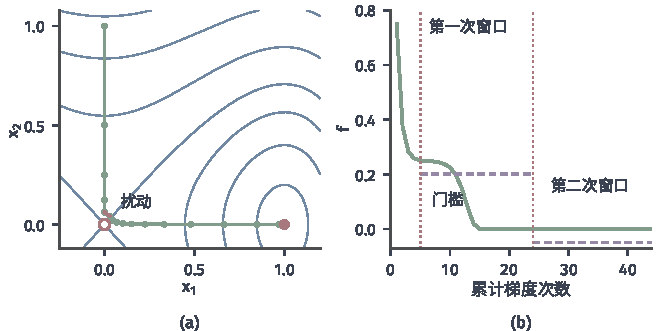
\includegraphics[width=112mm]{figures/05-optimization/02-smooth-optimization/matplotlib/saddle-pgd-run/figure.pdf}
  \caption{扰动梯度法在目标~\eqref{eq:saddle-example}上的运行，$T_{\mathrm{w}}=19$，$F=0.05$，$\bm{\xi}=(0.03,-0.02)$。(a)绿线是路径，红色短线是扰动。(b)目标值随累计梯度次数的变化，红色点线是触发扰动的时刻，紫色虚线是各窗口要求达到的门槛。第一次窗口越过门槛，第二次窗口没有。}
  \label{fig:saddle-pgd-run}
\end{BookInlineFigure}

\paragraph{一般目标上的保证}
定理~\ref{thm:saddle-quadratic-escape}只对二次目标成立。目标不是二次时，Hessian会随位置变化，放大过程可能被打断，所以需要Hessian的Lipschitz条件来控制窗口内的偏差。参数按下面的方式联合选取时，有如下保证\scite{jin2017escape}。

\begin{theorem}[扰动梯度法的高概率保证]
 \label{thm:saddle-pgd}
 设$f$下有界，$\nabla f$是$L$-Lipschitz的，$\nabla^2f$是$M$-Lipschitz的，$\Delta_f=f(\bm{x}^{(0)})-f_{\inf}$，$\varepsilon\leq L^2/M$。取$\alpha=1/L$，半径$r$、窗口$T_{\mathrm{w}}$和门槛$F$按$L,M,\varepsilon,\delta,n,\Delta_f$确定，则至少以$1-\delta$的概率，扰动梯度法返回的点满足
 \begin{equation}
  \lVert\nabla f(\tilde{\bm{x}})\rVert_2\leq\varepsilon,\qquad
  \lambda_{\min}\bigl(\nabla^2f(\tilde{\bm{x}})\bigr)\geq-\sqrt{M\varepsilon},
  \label{eq:saddle-pgd-guarantee}
 \end{equation}
 所用梯度次数为$\tilde O\bigl(L\Delta_f/\varepsilon^2\bigr)$，$\tilde O$隐去了$n,1/\delta,L,M,\Delta_f,1/\varepsilon$的多项对数因子。
\end{theorem}

证明的核心比二次情形多了一个技巧。不能再按特征分量独立讨论，于是考虑两条从窄带两侧出发、只在$\bm{q}_1$方向相差$2w$的迭代序列，用Hessian的Lipschitz条件证明它们的差在窗口内按指数增长，因此两条序列至少有一条离开基点足够远，目标也因此下降足够多。这说明“卡住”的初值不可能在$\bm{q}_1$方向上有大于$2w$的宽度，窄带的宽度得到了控制。完整论证篇幅较长，读者可查阅\scite{jin2017escape}。

定理对参数的要求是实质性的。扰动半径、窗口长度和门槛必须与$L$、$M$、$\varepsilon$和目标下降总量匹配。这里要区分两件事：结论说的是以高概率到达式~\eqref{eq:saddle-pgd-guarantee}定义的点，而不是找到局部极小点，更不是全局最优解。

\paragraph{严格鞍点的结论不能搬到退化驻点}
上面的论证依赖指数放大。退化驻点上没有负特征值，放大是多项式的。比较两个一元函数，步长取$\alpha=\tfrac12$：
\[
 -\frac12y^2:\quad y^{(t+1)}=\frac32y^{(t)};\qquad
 -\frac14y^4:\quad y^{(t+1)}=y^{(t)}+\frac12\bigl(y^{(t)}\bigr)^3.
\]

前者每步放大常数倍，从$y^{(0)}$到$0.5$只要$\log_{1.5}(0.5/y^{(0)})$步。后者可以用微分方程估计：$\mathrm{d}y/\mathrm{d}t\approx\tfrac12y^3$给出$1/y^2$随$t$线性减小，所需步数约为$1/(y^{(0)})^2$。从$y^{(0)}=0.01$出发，两者的实际步数分别是$10$和$10002$。图~\ref{fig:saddle-degenerate-escape}比较了这两种依赖。

\begin{BookInlineFigure}
  \centering
  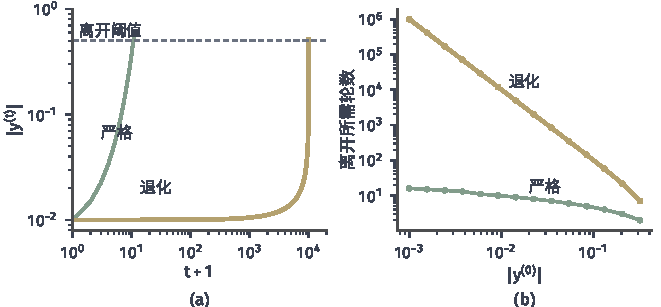
\includegraphics[width=112mm]{figures/05-optimization/02-smooth-optimization/matplotlib/saddle-degenerate-escape/figure.pdf}
  \caption{严格鞍点（绿，$-y^2/2$）与退化驻点（黄，$-y^4/4$）上步长$1/2$的梯度下降。(a)从$y^{(0)}=0.01$出发的$\lvert y^{(t)}\rvert$，虚线是离开阈值$0.5$。(b)离开所需轮数随初值大小的变化，严格鞍点按对数增长，退化驻点按$1/(y^{(0)})^2$增长。}
  \label{fig:saddle-degenerate-escape}
\end{BookInlineFigure}

在一个由$x_1^2-x_2^4$描述的退化鞍点上，扰动梯度法的窗口$T_{\mathrm{w}}$按严格鞍点设计，时间内分量几乎不长，窗口结束时目标没有明显下降，算法就返回基点。这并不违反定理~\ref{thm:saddle-pgd}：基点的$\lambda_{\min}=0\geq-\sqrt{M\varepsilon}$，它满足定理宣称的条件，只是这个条件本来就不排除退化鞍点。

\subsection{利用非正定模型}
\label{sec:saddle-indefinite-model}

二阶方法手里本来就有曲率矩阵。第~\ref{chap:second-order-methods}章和第~\ref{chap:trust-region}章对不定矩阵采取了两种态度：前者把矩阵修正成正定的，后者保留矩阵原样，用半径把模型关起来。这里比较两种态度在鞍点附近的差别，特别是哪种能利用负曲率。

\paragraph{信赖域模型怎样使用负曲率}
回顾第~\ref{chap:trust-region}章的子问题：
\begin{equation}
 \min_{\lVert\bm{p}\rVert_2\leq\Delta}\ m(\bm{p})=f(\bm{x})+\langle\bm{g},\bm{p}\rangle+\frac12\bm{p}^\top\bm{B}\bm{p}.
 \label{eq:saddle-tr-subproblem}
\end{equation}
$\bm{p}$是全局解的充要条件是存在$\lambda\geq0$，使
\begin{equation}
 (\bm{B}+\lambda\bm{I})\bm{p}=-\bm{g},\qquad
 \bm{B}+\lambda\bm{I}\succeq\bm{0},\qquad
 \lambda\bigl(\Delta-\lVert\bm{p}\rVert_2\bigr)=0.
 \label{eq:saddle-tr-optimality}
\end{equation}

第二个条件说明$\lambda\geq-\lambda_{\min}(\bm{B})$。所以$\bm{B}$不定时$\lambda>0$，解一定在边界上：模型沿负曲率方向一直下降，直到碰上半径。这里没有把任何曲率改成正值，负曲率被直接转化成一个长度为$\Delta$的步。

在原点取$\bm{B}=\operatorname{diag}(-1,1)$，$\Delta=\tfrac12$，$\bm{g}=\bm{0}$。条件~\eqref{eq:saddle-tr-optimality}给出$\lambda=1$，第一个方程$(\bm{B}+\bm{I})\bm{p}=\bm{0}$只约束$p_2=0$，于是
\[
 \bm{p}=\begin{bmatrix}\pm\tfrac12\\0\end{bmatrix},\qquad
 m(\bm{0})-m(\bm{p})=\frac18.
\]

代回目标，实际下降和两者之比分别是
\[
 f(\bm{0})-f\bigl(\tfrac12,0\bigr)=\frac14-\frac{9}{64}=0.1094,\qquad
 \rho=\frac{0.1094}{0.125}\approx0.875.
\]
这一步可以接受。梯度精确为零，信赖域仍然走出了一大步，这是只靠梯度的方法做不到的。

\paragraph{修正Hessian的用途不同}
第~\ref{chap:second-order-methods}章的修正让矩阵变成$\bm{B}=\bm{H}+\bm{E}\succ\bm{0}$，解$\bm{B}\bm{d}=-\bm{g}$，目的是得到下降方向，让线搜索有效。这时$\bm{g}=\bm{0}$意味着$\bm{d}=\bm{0}$，算法原地不动。

$\bm{g}$很小但不为零时，以谱修正为例，方向沿$\bm{q}_i$的分量是$-\langle\bm{g},\bm{q}_i\rangle/\lvert\lambda_i\rvert$，长度正比于梯度，鞍点附近很短。下面在点$(0.01,0.0625)$上比较两者。由式~\eqref{eq:saddle-example-derivatives}，该点的数据是
\[
 \bm{g}\approx\begin{bmatrix}-0.0100\\0.0625\end{bmatrix},\qquad
 \bm{H}\approx\operatorname{diag}(-0.9997,1).
\]

谱修正取绝对值，得到的方向和$\Delta=\tfrac12$时子问题的解分别是
\[
 \bm{d}\approx\begin{bmatrix}0.0100\\-0.0625\end{bmatrix},\qquad
 \bm{p}\approx\begin{bmatrix}0.4990\\-0.0309\end{bmatrix}.
\]

子问题的$\lambda\approx1.020$，预测下降$0.1309$，实际下降$0.1142$，$\rho\approx0.872$，接受。修正方向沿$x_1$的分量只有子问题解的约$2\%$。图~\ref{fig:saddle-tr-modified}(a)画出了这两个方向，(b)比较后续运行：修正方法配回溯时，$x_1$大约每轮翻一倍，要$6$轮才接近$0.77$；信赖域$3$轮之内就到了谷底附近，其间有一次拒绝。

\begin{BookInlineFigure}
  \centering
  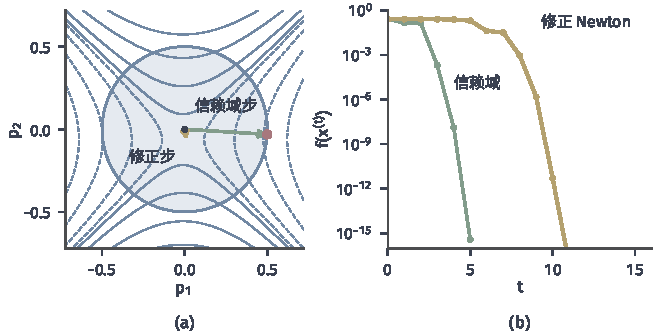
\includegraphics[width=112mm]{figures/05-optimization/02-smooth-optimization/matplotlib/saddle-tr-modified/figure.pdf}
  \caption{点$(0.01,0.0625)$处的比较。(a)蓝线是二次模型的等高线（虚线为负值），浅蓝圆盘半径$\Delta=1/2$，绿色箭头指向子问题的解（红点），黄色短箭头是谱修正方向。(b)从该点出发目标值随轮数的变化，绿线是精确求解子问题的信赖域，黄线是谱修正加Armijo回溯。}
  \label{fig:saddle-tr-modified}
\end{BookInlineFigure}

\paragraph{梯度与负曲率方向正交时}
最能说明两种方法差别的是$\langle\bm{g},\bm{q}_1\rangle=0$的情形。在点$(0,0.0625)$，梯度是$(0,0.0625)$，与$\bm{e}_1$正交。此时条件~\eqref{eq:saddle-tr-optimality}的第一行变成$(\lambda-1)p_1=0$，半正定条件要求$\lambda\geq1$。取$\lambda=1$，第二行和球面条件给出
\[
 p_2=-\frac{0.0625}{1+1}=-0.03125,\qquad
 p_1=\pm\sqrt{\Delta^2-p_2^2}\approx\pm0.4990.
\]

这是第~\ref{chap:trust-region}章所说的困难情形：$\bm{B}+\lambda\bm{I}$奇异，方程本身不能确定$p_1$，要沿$\bm{q}_1$方向补一个分量才到达边界。这一步的预测下降是$0.1260$，$\rho\approx0.877$。

截断共轭梯度却看不到$\bm{e}_1$。它的迭代只在由$\bm{g}$生成的Krylov子空间中进行，这里就是$x_2$轴，第一步就到达$(0,-0.0625)$，残差为零而停止，预测下降只有约$0.002$。图~\ref{fig:saddle-tr-hard-case}(a)是这个点上的模型，(b)是从$(0,1)$出发的运行。截断共轭梯度第一步到达原点，$\bm{g}=\bm{0}$，算法宣布完成。精确子问题第一步是$(0.866,-0.5)$，比值$\rho=0.8125$，第二步到达$(1.039,0)$。

\begin{BookInlineFigure}
  \centering
  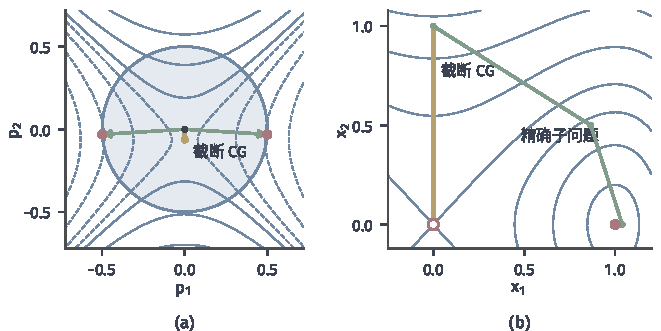
\includegraphics[width=112mm]{figures/05-optimization/02-smooth-optimization/matplotlib/saddle-tr-hard-case/figure.pdf}
  \caption{困难情形。(a)点$(0,0.0625)$处的模型（蓝线）与半径$1/2$的圆盘，两个红点是子问题的全局解，黄线是截断共轭梯度的结果，它留在$p_2$轴上。(b)从$(0,1)$出发、$\Delta^{(0)}=1$的运行：绿线精确求解子问题，黄线用截断共轭梯度，一步到达鞍点后停止。}
  \label{fig:saddle-tr-hard-case}
\end{BookInlineFigure}

这里要记住：算出的步是否利用负曲率，由子问题的求解方式决定。使用截断共轭梯度的信赖域，在$\bm{g}$恰好避开$\bm{q}_1$时和修正方法一样看不见负曲率。

\paragraph{后续保证的差别}
第~\ref{chap:trust-region}章的二阶保证要求候选步的模型下降满足下面的条件，其中$\lambda_-=\max\{0,-\lambda_{\min}\}$，$c_2>0$是常数：
\[
 \operatorname{pred}(\bm{p})\geq c_2\lambda_-\Delta^2.
\]
由此得到
\begin{equation}
 \liminf_{t\to\infty}\max\bigl\{\lVert\bm{g}^{(t)}\rVert_2,\ \lambda_-^{(t)}\bigr\}=0.
 \label{eq:saddle-tr-liminf}
\end{equation}
精确解$c_2=\tfrac12$，满足这一条；只有一阶信息的步不满足，保证也就退回到$\bm{g}^{(t)}\to\bm{0}$。

不想精确求解时，可以把第~\ref{sec:saddle-detection}节的检测嫁接进来。设检测给出$\bm{v}$，$\bm{v}^\top\bm{B}\bm{v}\leq-\gamma$，选符号使$\langle\bm{g},\bm{v}\rangle\leq0$，把$\Delta\bm{v}$作为候选步，它的预测下降是
\[
 m(\bm{0})-m(\Delta\bm{v})=-\Delta\langle\bm{g},\bm{v}\rangle-\frac{\Delta^2}{2}\bm{v}^\top\bm{B}\bm{v}\geq\frac12\gamma\Delta^2.
\]

只要$\gamma$不小于$\lambda_-$的一个固定倍数，例如$\gamma\geq\tfrac12\lambda_-$，就得到$c_2=\tfrac14$，第~\ref{chap:trust-region}章的论证可以照搬。当然这样一来保证就带上了检测的失败概率。表~\ref{tab:saddle-model-compare}总结了各种做法的区别。

\begin{BookInlineTable}
  \centering
  \begin{tabular}{@{}lll@{}}
    \toprule
    做法 & 在$\bm{g}=\bm{0}$的鞍点 & 结论\\
    \midrule
    修正Hessian加线搜索 & 不动 & $\bm{g}^{(t)}\to\bm{0}$\\
    信赖域，Cauchy步或截断CG & 不动 & $\bm{g}^{(t)}\to\bm{0}$\\
    信赖域，精确子问题 & 走到边界 & 式~\eqref{eq:saddle-tr-liminf}\\
    信赖域，加入负曲率检测 & 走到边界 & 同上，带失败概率\\
    \bottomrule
  \end{tabular}
  \caption{几种处理不定矩阵的做法。式~\eqref{eq:saddle-tr-liminf}的二阶结论只说明子列满足二阶必要条件，不说明极限点是局部极小点。}
  \label{tab:saddle-model-compare}
\end{BookInlineTable}

总之，修正Hessian解决的是“方向要下降”，保留不定模型解决的是“负曲率要被利用”。两者的出发点不同，后续能给出的保证也不同，不应混为一谈。


\section{停止条件与计算成本}
\label{sec:saddle-stopping}

算法什么时候可以停，一次运行究竟可以报告什么？第~\ref{chap:smooth-foundations}章要求比较算法之前固定三件事：误差标准、返回哪个点、计算量怎样累计。这里把这三件事放到二阶情形下落实。

\paragraph{两个容差}
只有一个梯度容差无法排除鞍点，所以要同时控制梯度大小和Hessian最小特征值的负部。

\begin{definition}[近似二阶驻点]
 \label{def:saddle-approximate}
 给定$\varepsilon_g>0$，$\varepsilon_H>0$，若点$\bm{x}$满足
 \begin{equation}
  \lVert\nabla f(\bm{x})\rVert_2\leq\varepsilon_g,\qquad
  \lambda_{\min}\bigl(\nabla^2f(\bm{x})\bigr)\geq-\varepsilon_H,
  \label{eq:saddle-approximate}
 \end{equation}
 就称它为$(\varepsilon_g,\varepsilon_H)$\term{近似二阶驻点}（approximate second-order stationary point）。
\end{definition}

例中$\varepsilon_g=0.1$，$\varepsilon_H\approx0.775$。点$(0,0.0625)$的梯度范数$0.0625$通过了第一个条件，$\lambda_{\min}=-1$没有通过第二个。点$(0.9686,0.0039)$的梯度范数$0.060$，$\lambda_{\min}=1$，两个都通过。图~\ref{fig:saddle-tolerance-plane}(a)把表~\ref{tab:saddle-nc-run}的运行画在这两个量组成的平面上，(b)在变量空间中画出了两种验收区的差别。

\begin{BookInlineFigure}
  \centering
  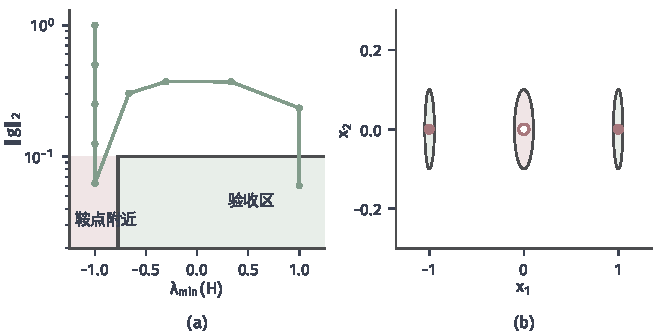
\includegraphics[width=112mm]{figures/05-optimization/02-smooth-optimization/matplotlib/saddle-tolerance-plane/figure.pdf}
  \caption{两个容差的验收区，$\varepsilon_g=0.1$，$\varepsilon_H\approx0.775$。(a)横轴是$\lambda_{\min}(\bm{H})$，纵轴是$\lVert\bm{g}\rVert_2$（对数坐标），绿色矩形是验收区，粗线是边界，浅红区梯度合格而曲率不合格，折线是表~\ref{tab:saddle-nc-run}的运行。(b)目标~\eqref{eq:saddle-example}上$\lVert\nabla f\rVert_2\leq\varepsilon_g$的三块区域，鞍点周围的一块（浅红）不满足曲率条件，只有两侧（浅绿）满足全部条件。}
  \label{fig:saddle-tolerance-plane}
\end{BookInlineFigure}

\paragraph{两个容差怎样搭配}
两个容差不是独立的。式~\eqref{eq:saddle-approximate}对目标下降的限制可以由三次上界直接算出：设半径$r$的球落在引理~\ref{lem:saddle-cubic}的凸集内，对$\lVert\bm{p}\rVert_2\leq r$，由该引理和式~\eqref{eq:saddle-approximate}，
\begin{equation}
 f(\bm{x}+\bm{p})\geq f(\bm{x})-\varepsilon_gr-\frac12\varepsilon_Hr^2-\frac{M}{6}r^3.
 \label{eq:saddle-tolerance-drop}
\end{equation}

三项分别来自梯度、负曲率和Hessian的变化。让三项同量级，由后两项得到$r\sim\varepsilon_H/M$，代入前两项得到$\varepsilon_g\sim\varepsilon_H^2/M$，于是自然的搭配是
\begin{equation}
 \varepsilon_H=\sqrt{M\varepsilon_g}.
 \label{eq:saddle-tolerance-scale}
\end{equation}

此时取$r=\sqrt{\varepsilon_g/M}$，式~\eqref{eq:saddle-tolerance-drop}的三项合计给出
\[
 f(\bm{x}+\bm{p})\geq f(\bm{x})-\frac{5}{3}\frac{\varepsilon_g^{3/2}}{\sqrt{M}}.
\]
这就是通过验收的点能保证的事：在半径$r$的球内，目标至多还能下降这么多。

\paragraph{通过验收不等于局部极小}
式~\eqref{eq:saddle-tolerance-drop}只限制了小球内的下降幅度，并不排除下降。$x_1^2-x_2^4$在原点梯度和Hessian的负部都是零，对任意容差都通过验收，而原点不是局部极小点，甚至这个目标没有下界。

容差取得过大也会放过严格鞍点。例中若$\varepsilon_H=2$，原点的$\lambda_{\min}=-1$就能通过。

所以报告结果时，应该写“近似二阶驻点，容差为$(\varepsilon_g,\varepsilon_H)$”，不写“找到了局部极小点”，更不写“找到了最优解”。

\paragraph{返回哪个点}
验收条件是针对具体的点的，所以返回的点必须就是验收的那个点。负曲率算法直接返回验收通过的$\bm{x}^{(t)}$。扰动梯度法返回窗口开始之前保存的基点$\tilde{\bm{x}}$，因为梯度小的判断是在基点上作出的，窗口结束时的点没有经过判断。

\paragraph{要累计哪些计算量}
这一节的成本有四类，单位要分开：梯度次数，Hessian向量积次数，矩阵分解次数，以及扰动窗口的梯度次数。

扰动窗口的次数也有上界。除了最后一次之外，每次窗口都使目标下降至少$F$，所以窗口总数不超过$\Delta_f/F+1$。例中上界是$16$次窗口，共$304$次梯度，实际只用了$2$次窗口。每次窗口都有失败的可能，失败概率要像下面的检测一样累计。

检测的失败概率也要累计。负曲率算法可能进行多次检测，任何一次“未找到”判断错误都会使算法提前停止。若检测次数不超过$K$，每次失败概率取$\delta/K$，由并的概率不等式，总失败概率不超过$\delta$，代价只是对数因子$\ln(K/\delta)$。

检测有两个方向，失败只发生在“未找到”的方向上。每次发现负曲率都是确定的，所以不需要担心算法走错一步。真正的风险是错误地宣布停止。下面把这些成本组合起来。

取$\gamma_0=\varepsilon_H/2$，检测精度$\varepsilon_H/2$，由式~\eqref{eq:saddle-no-find}，未找到时$\lambda_{\min}\geq-\varepsilon_H$。把$\varepsilon_H=\sqrt{M\varepsilon}$代入定理~\ref{thm:saddle-nc-count}，负曲率步的次数不超过
\begin{equation}
 K=\frac{12\sqrt{M}\,\Delta_f}{\varepsilon^{3/2}}.
 \label{eq:saddle-detect-count}
\end{equation}

用Lanczos方法时每次检测$O(\sqrt{L/\varepsilon_H}\,\ln(nK/\delta))$次乘积，总数是
\begin{equation}
 O\Bigl(\frac{\sqrt{L}\,M^{1/4}\Delta_f}{\varepsilon^{7/4}}\ln\frac{nK}{\delta}\Bigr).
 \label{eq:saddle-lanczos-total}
\end{equation}
这个量对$1/\varepsilon$的幂次比梯度步的$O(L\Delta_f/\varepsilon^2)$低$1/4$，所以在小容差下乘积的总量不会超过梯度的总量。换成幂迭代时，每次检测$O((L/\varepsilon_H)\ln(nK/\delta))$次乘积，总数变成$O((L\Delta_f/\varepsilon^2)\ln(nK/\delta))$，与梯度步同阶。

表~\ref{tab:saddle-cost-bounds}汇总了各种做法在最坏情形下的曲率成本，表中$\varepsilon_g=\varepsilon$，$\varepsilon_H=\sqrt{M\varepsilon}$。前三行的梯度次数都不超过$2L\Delta_f/\varepsilon^2$加检测带来的少量读取，扰动梯度法的梯度次数是$\tilde O(L\Delta_f/\varepsilon^2)$，这里的$\tilde O$隐去了对数因子。

\begin{BookInlineTable}
  \centering
  \begin{tabular}{@{}lll@{}}
    \toprule
    方法 & 曲率读取（梯度次数见正文） & 保证\\
    \midrule
    梯度下降 & 无 & 一阶，确定\\
    负曲率步，特征分解 & $O(\sqrt{M}\Delta_f/\varepsilon^{3/2})$次分解 & 二阶，确定\\
    负曲率步，Lanczos & 式~\eqref{eq:saddle-lanczos-total}的次数 & 二阶，$\geq1-\delta$\\
    扰动梯度法 & 无 & 二阶，$\geq1-\delta$\\
    信赖域，精确子问题 & $O(\varepsilon^{-2})$轮，每轮一次分解 & 二阶，确定\\
    \bottomrule
  \end{tabular}
  \caption{达到式~\eqref{eq:saddle-approximate}的最坏情形成本，“二阶”指近似二阶驻点，“$\geq1-\delta$”指成立的概率。信赖域一行由第~\ref{chap:trust-region}章的轮数估计得到，并依赖半径下界中的常数。}
  \label{tab:saddle-cost-bounds}
\end{BookInlineTable}

\paragraph{一次实际运行的账}
上界比较的是最坏情形，单次运行要按实际次数报告。表~\ref{tab:saddle-run-cost}是从$(0,1)$出发、$\varepsilon_g=0.1$、$\varepsilon_H\approx0.775$时各方法的实际计数。

\begin{BookInlineTable}
  \centering
  \begin{tabular}{@{}lrlcc@{}}
    \toprule
    方法 & 梯度 & 曲率读取 & 返回点 & 通过\\
    \midrule
    梯度下降 & $5$ & 无 & $(0,\ 0.0625)$ & 否\\
    谱修正Newton & $2$ & $1$次分解 & $(0,\ 0)$ & 否\\
    信赖域，截断CG & $2$ & $1$次乘积 & $(0,\ 0)$ & 否\\
    负曲率步，特征分解 & $10$ & $2$次分解 & $(0.969,\ 0.004)$ & 是\\
    负曲率步，幂迭代 & $11$ & $151$次乘积 & $(0.981,\ -0.001)$ & 是\\
    扰动梯度法 & $44$ & 无 & $(1.000,\ 0.000)$ & 是\\
    信赖域，精确子问题 & $3$ & $3$次分解 & $(1.039,\ 0)$ & 是\\
    \bottomrule
  \end{tabular}
  \caption{从$(0,1)$出发的实际计数，“通过”指是否满足式~\eqref{eq:saddle-approximate}。幂迭代用$L=2$，随机起点的种子固定为$0$，检测精度$\varepsilon_H/2$，失败概率$\delta=0.05$（两次检测的总失败概率约$0.1$），上限由式~\eqref{eq:saddle-power-rounds}算得$149$次。}
  \label{tab:saddle-run-cost}
\end{BookInlineTable}

表中前三行的算法都很便宜，但报告的点是鞍点。它们的共同问题是起点在$x_2$轴上，梯度始终看不到$x_1$方向。负曲率步用幂迭代时，第一次检测只用$2$次乘积就找到了方向，其余$149$次全部花在最后一次“未找到”的确认上。

这说明确认“没有负曲率”才是最贵的一步，手段越便宜，这一步越依赖概率。实际程序常常把上限设得比理论值小，这时要如实报告：这样的结果只是经验判断，不再带有定理~\ref{thm:saddle-power}的概率保证。

\paragraph{一次报告应该包含什么}
把三件事落实到底，一次运行的结论可以写成这样：对目标~\eqref{eq:saddle-example}，从$(0,1)$出发，用幂迭代检测负曲率的交替算法，返回点满足$\lVert\nabla f\rVert_2\leq0.1$；未找到负曲率的判断由$149$次乘积支持，至少以$0.9$的概率有$\lambda_{\min}\geq-0.775$；共用$11$次梯度和$151$次Hessian向量积。

这样的报告说清了误差标准（两个容差）、返回的点（验收通过的点）、成本（分类计数）和可信度（失败概率）。它没有声称局部极小，也没有声称全局最优，这两件事本章的方法都保证不了。


\section{本章小结}
\label{sec:saddle-summary}

本章从一个具体的疑问出发：梯度很小的点算不算找到了解。梯度小只说明一阶变化弱，山口和谷底都满足这一点。

驻点按二阶信息分成严格鞍点和二阶驻点。负曲率是确凿的证据，说明这里还能下降；Hessian正定也是确凿的证据，说明这里是局部极小点。半正定而奇异的情形，二阶信息无法判断，$x_1^2+x_2^4$与$x_1^2-x_2^4$就是例子。即使确实是局部极小点，也不说明是全局最优解。

负曲率可以只靠Hessian向量积发现。幂迭代和Lanczos方法从随机起点出发，找到方向时的结论是确定的，未找到时的结论带有失败概率，检测误差和差分误差都要计入。

离开鞍点有三种机制，它们的条件和结论各不相同。

\begin{BookInlineTable}
  \centering
  \begin{tabular}{@{}lll@{}}
    \toprule
    机制 & 需要的条件 & 结论\\
    \midrule
    负曲率步 & 方向、Hessian Lipschitz & 每步确定下降$\frac{2\gamma^3}{3M^2}$\\
    扰动梯度法 & 梯度、$L$、$M$、随机扰动 & 高概率到达近似二阶驻点\\
    不定模型 & 子问题使用负曲率 & 二阶必要条件的下极限\\
    \bottomrule
  \end{tabular}
  \caption{三种离开鞍点的机制。修正Hessian只为得到下降方向，它的保证停留在一阶。}
  \label{tab:saddle-summary}
\end{BookInlineTable}

检测精度和离开机制共同决定了能够声称的保证。停止时用两个容差描述近似二阶驻点，$\varepsilon_H=\sqrt{M\varepsilon_g}$是自然的搭配，它限制了小球内还能下降多少，但不说明这个点是局部极小点。计算量要把梯度、Hessian向量积、分解和扰动窗口分开统计，并报告确定性保证或相应的失败概率。

到这里，光滑优化中的方向、步长、曲率和成本的框架已经完整。这些方法都假设梯度存在。下一部分研究目标在某些点没有普通梯度时，怎样改用次微分和邻近结构。

